\documentclass{article}

\usepackage[a4paper]{geometry}
\usepackage[spanish]{babel}
\usepackage{xcolor}
\usepackage{placeins}

\usepackage{mathbbol}
\usepackage{amsmath}
\usepackage{amsfonts}
\usepackage{hyperref}
\usepackage{graphicx}
\usepackage{subcaption}

\usepackage{algorithm}
\usepackage{algpseudocode}

% Cambiar 'Cuadro' -> 'Tabla'
\addto\captionsspanish{
    \renewcommand{\tablename}{Tabla}
}

\begin{document}

\begin{center}
    {\Large Aprendizaje Automático para Datos en Grafos} \\
    {\LARGE \textbf{Laboratorio 3}} \\
    \vspace{2em}
    \begin{minipage}{0.45\textwidth}
        \centering
        Graciana Castro \\
        4.808.848-2 \\
        gcastro@fing.edu.uy
    \end{minipage}
    \hfill
    \begin{minipage}{0.45\textwidth}
        \centering
        Julian O'Flaherty \\
        6.285.986-9 \\
        julian.o.flaherty@fing.edu.uy
    \end{minipage}
\end{center}


\section{Introducción}

\section{Grafos Erdös-Rényi}

Los grafos \emph{Erdös-Rényi}\cite{erdos1959random} (ER) son grafos aleatorios con un algoritmo de generación muy simple, donde
a cada par de nodos se le asigna una arista con una probabilidad $p$. Pese a la simplicidad del algoritmo,
los grafos ER tienen propiedades interesantes. Una de estas propiedades es que si 
\begin{equation}
    \label{eq:er_threshold_1}
    p > \frac{(1 + \epsilon)ln(n)}{n} \quad\quad \epsilon > 0
\end{equation}
entonces la probabilidad de que el grafo sea conexo es practicamente 1. Analogamente,
si 
\begin{equation}
    \label{eq:er_threshold_2}
    p < \frac{(1 - \epsilon)ln(n)}{n} \quad\quad \epsilon > 0
\end{equation}
entonces la probabilidad de que el grafo sea conexo es practicamente 0.

\begin{figure}[htb]
    \centering
    \begin{subfigure}{\textwidth}
        \centering
        \begin{minipage}{0.32\textwidth}
            \centering
            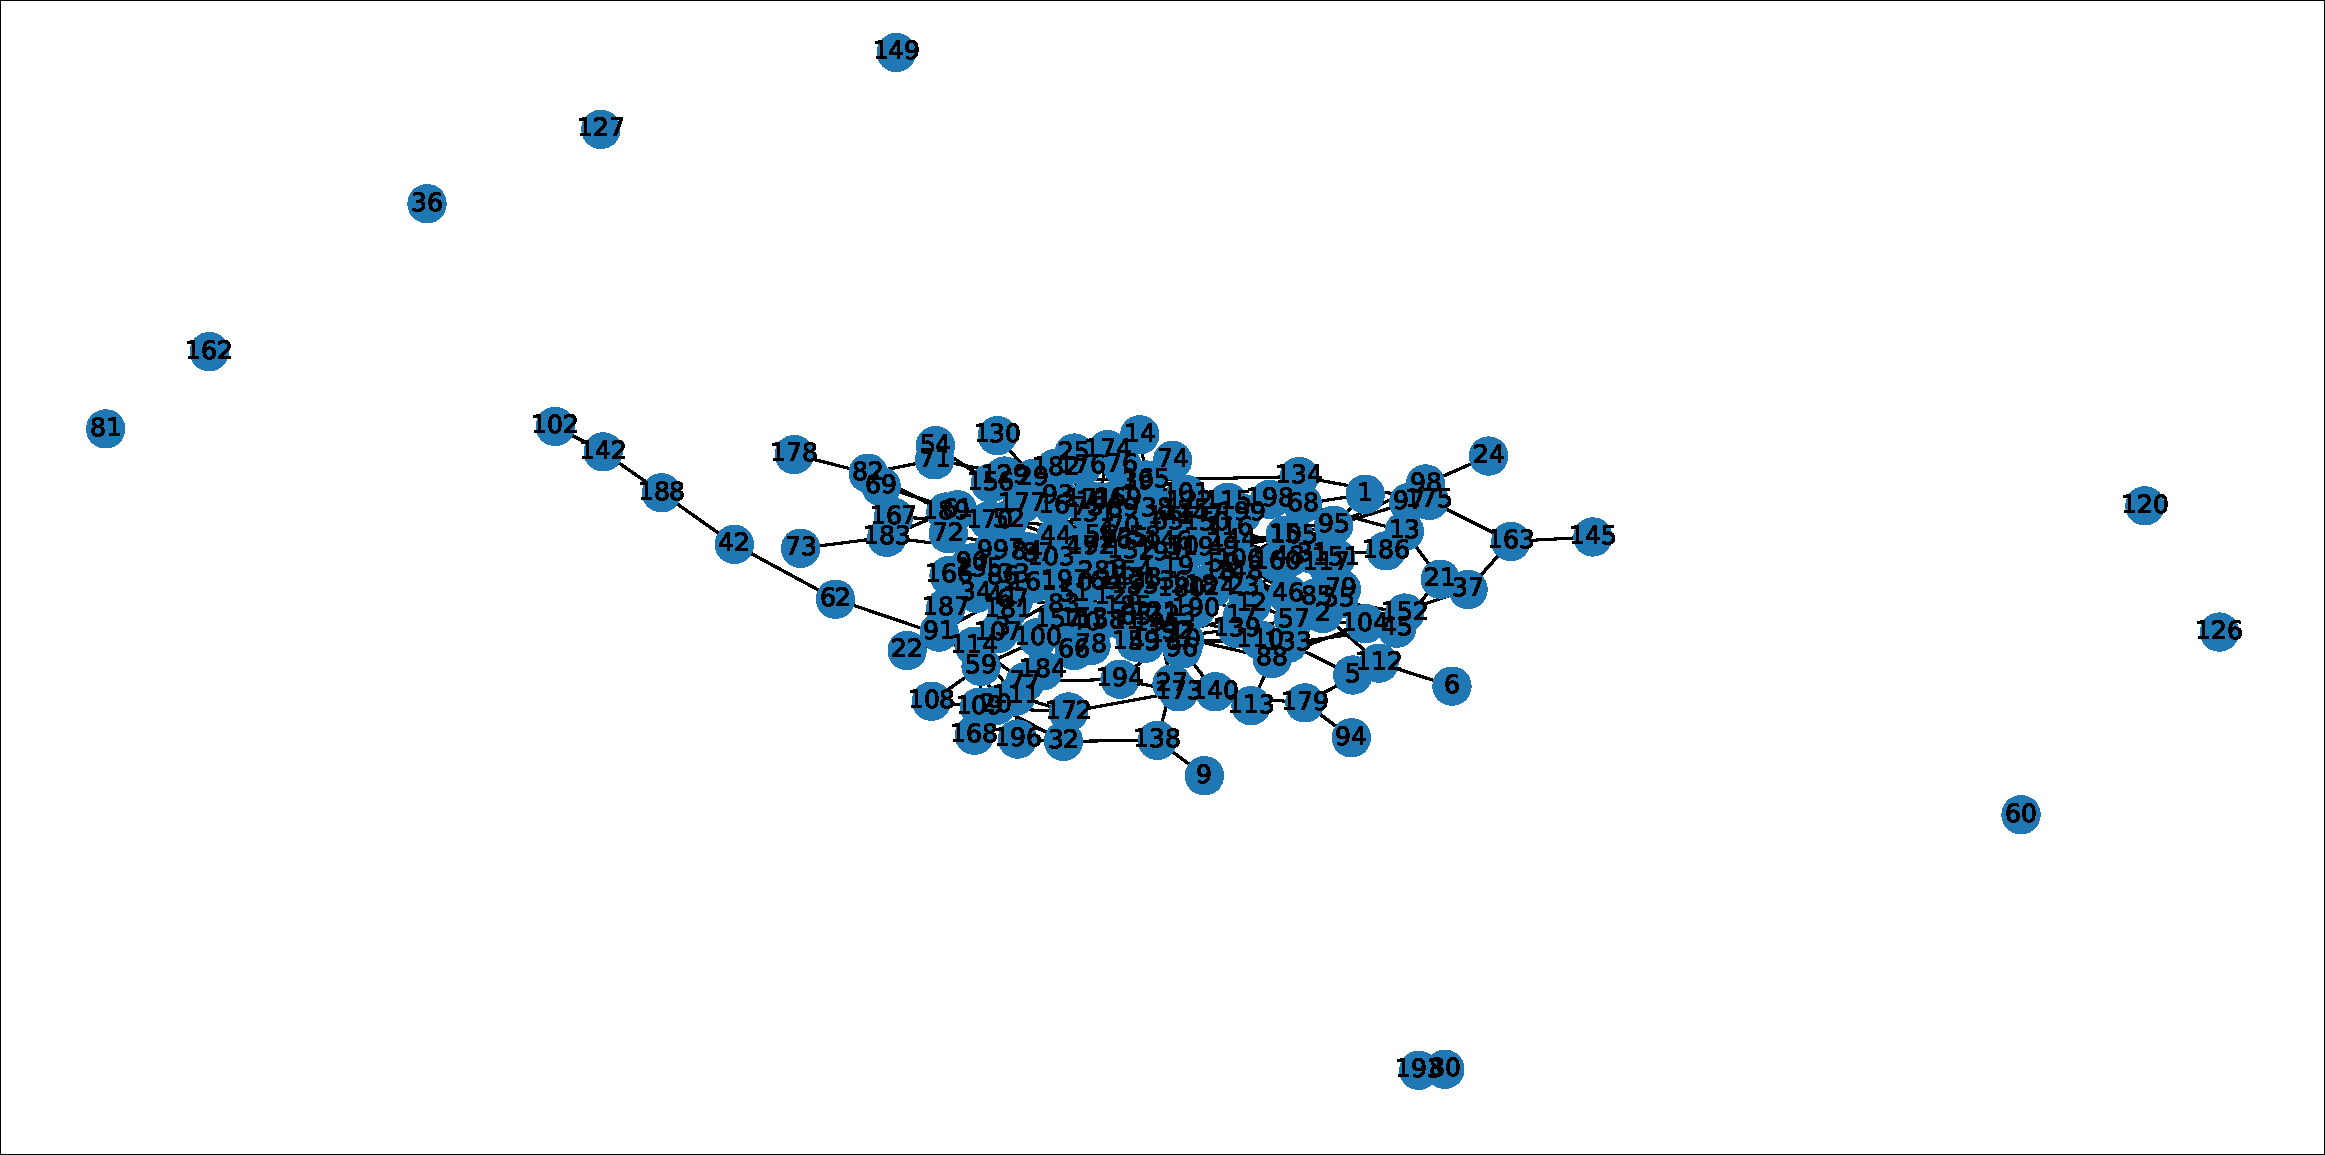
\includegraphics[width=\linewidth]{images/erdos_renyi/n200_p0.016491586832740178_0.pdf}
        \end{minipage}\hfill
        \begin{minipage}{0.32\textwidth}
            \centering
            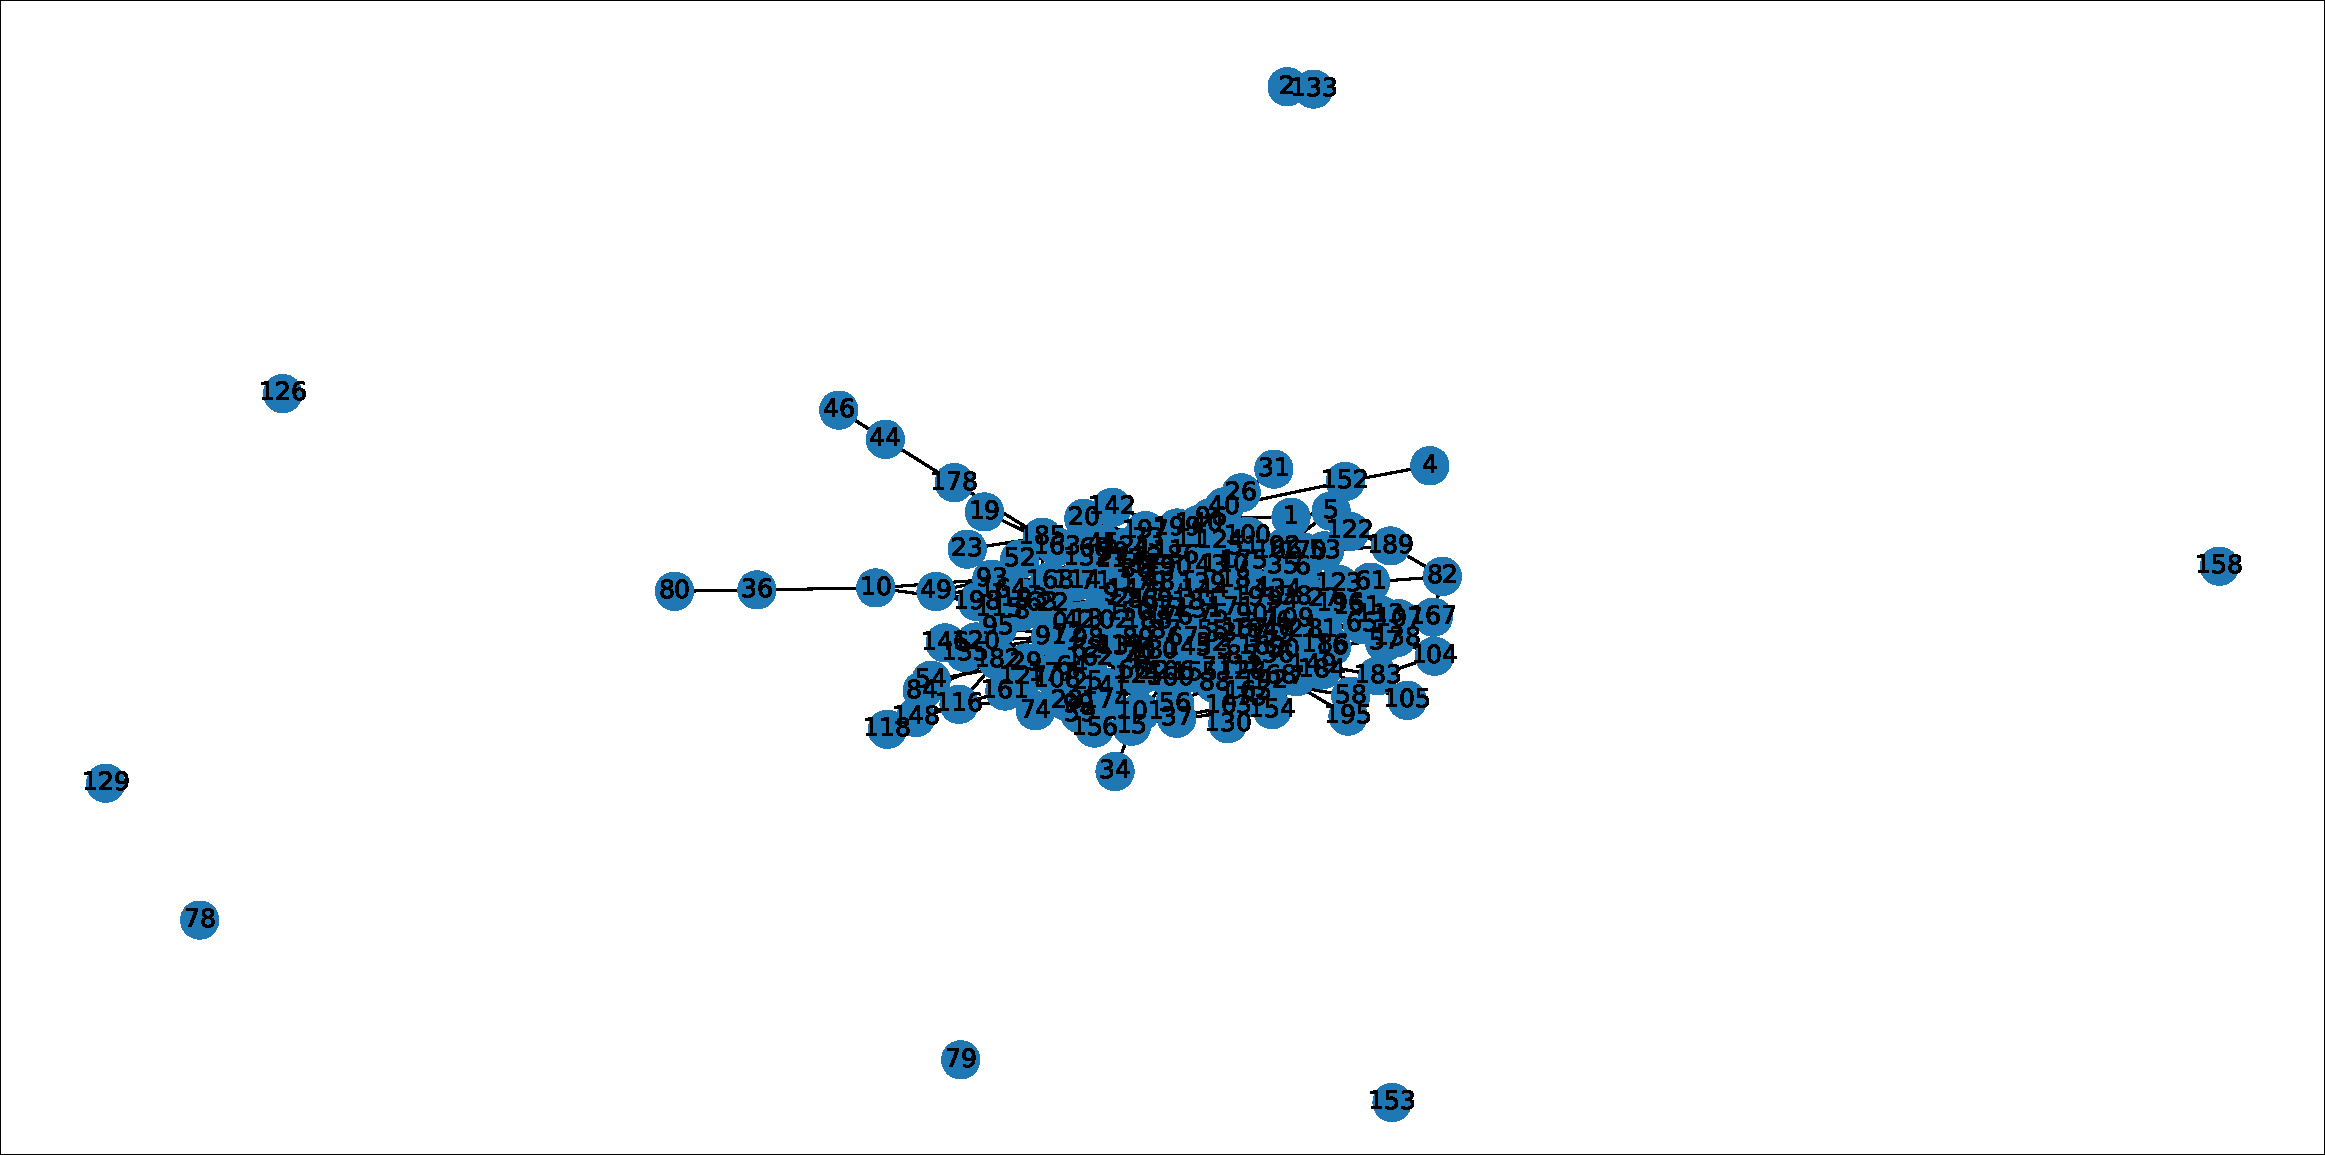
\includegraphics[width=\linewidth]{images/erdos_renyi/n200_p0.016491586832740178_1.pdf}
        \end{minipage}\hfill
        \begin{minipage}{0.32\textwidth}
            \centering
            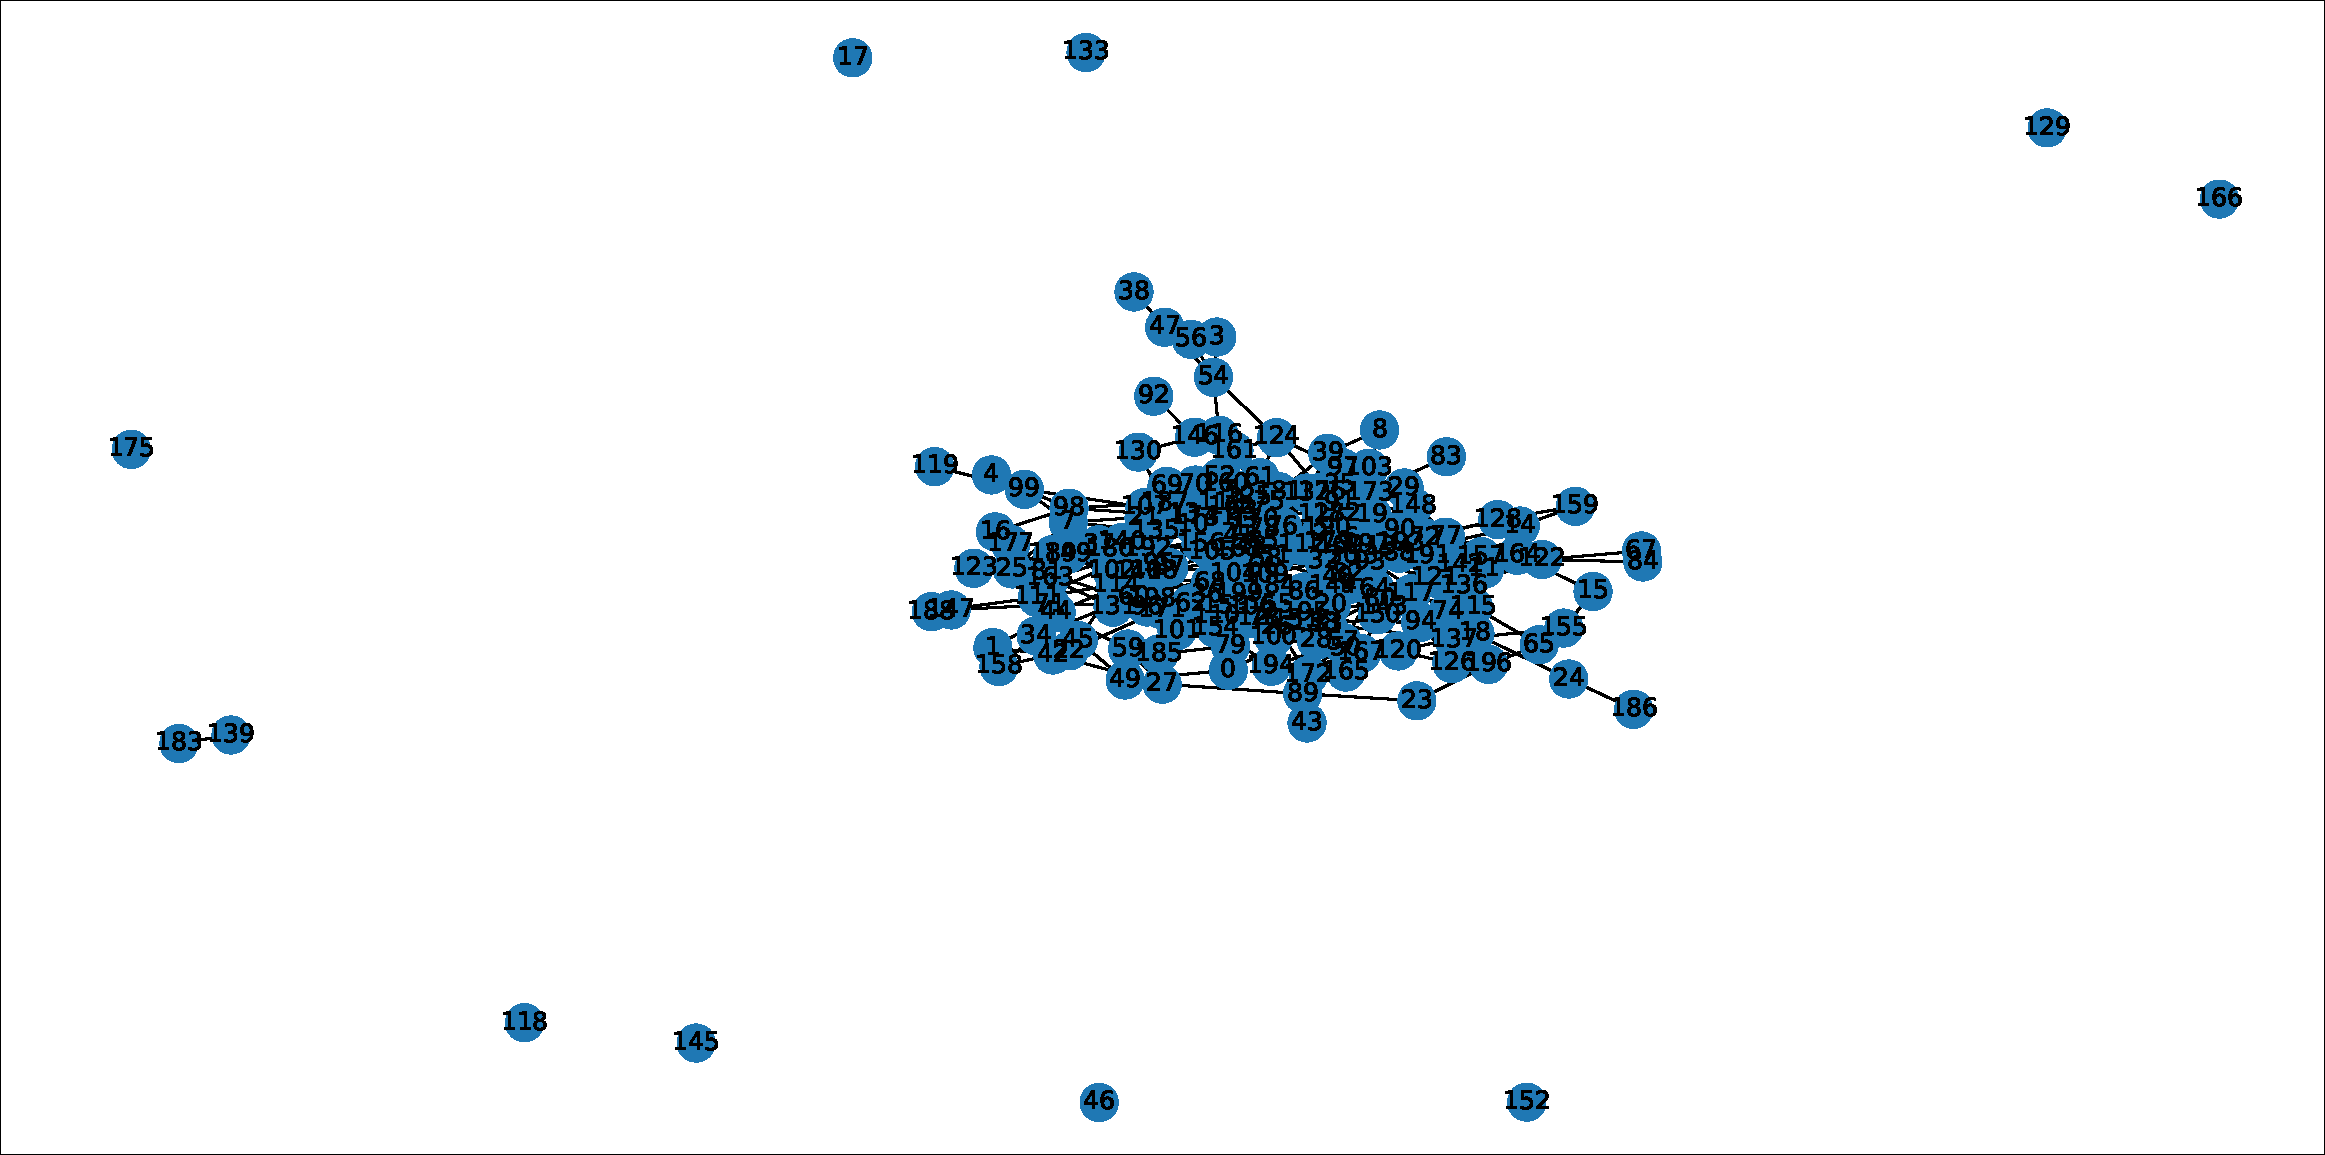
\includegraphics[width=\linewidth]{images/erdos_renyi/n200_p0.016491586832740178_2.pdf}
        \end{minipage}
        \caption{$n=200$, $p=0.01649$}
    \end{subfigure}

    \par\bigskip

    \begin{subfigure}{\textwidth}
        \centering
        \begin{minipage}{0.32\textwidth}
            \centering
            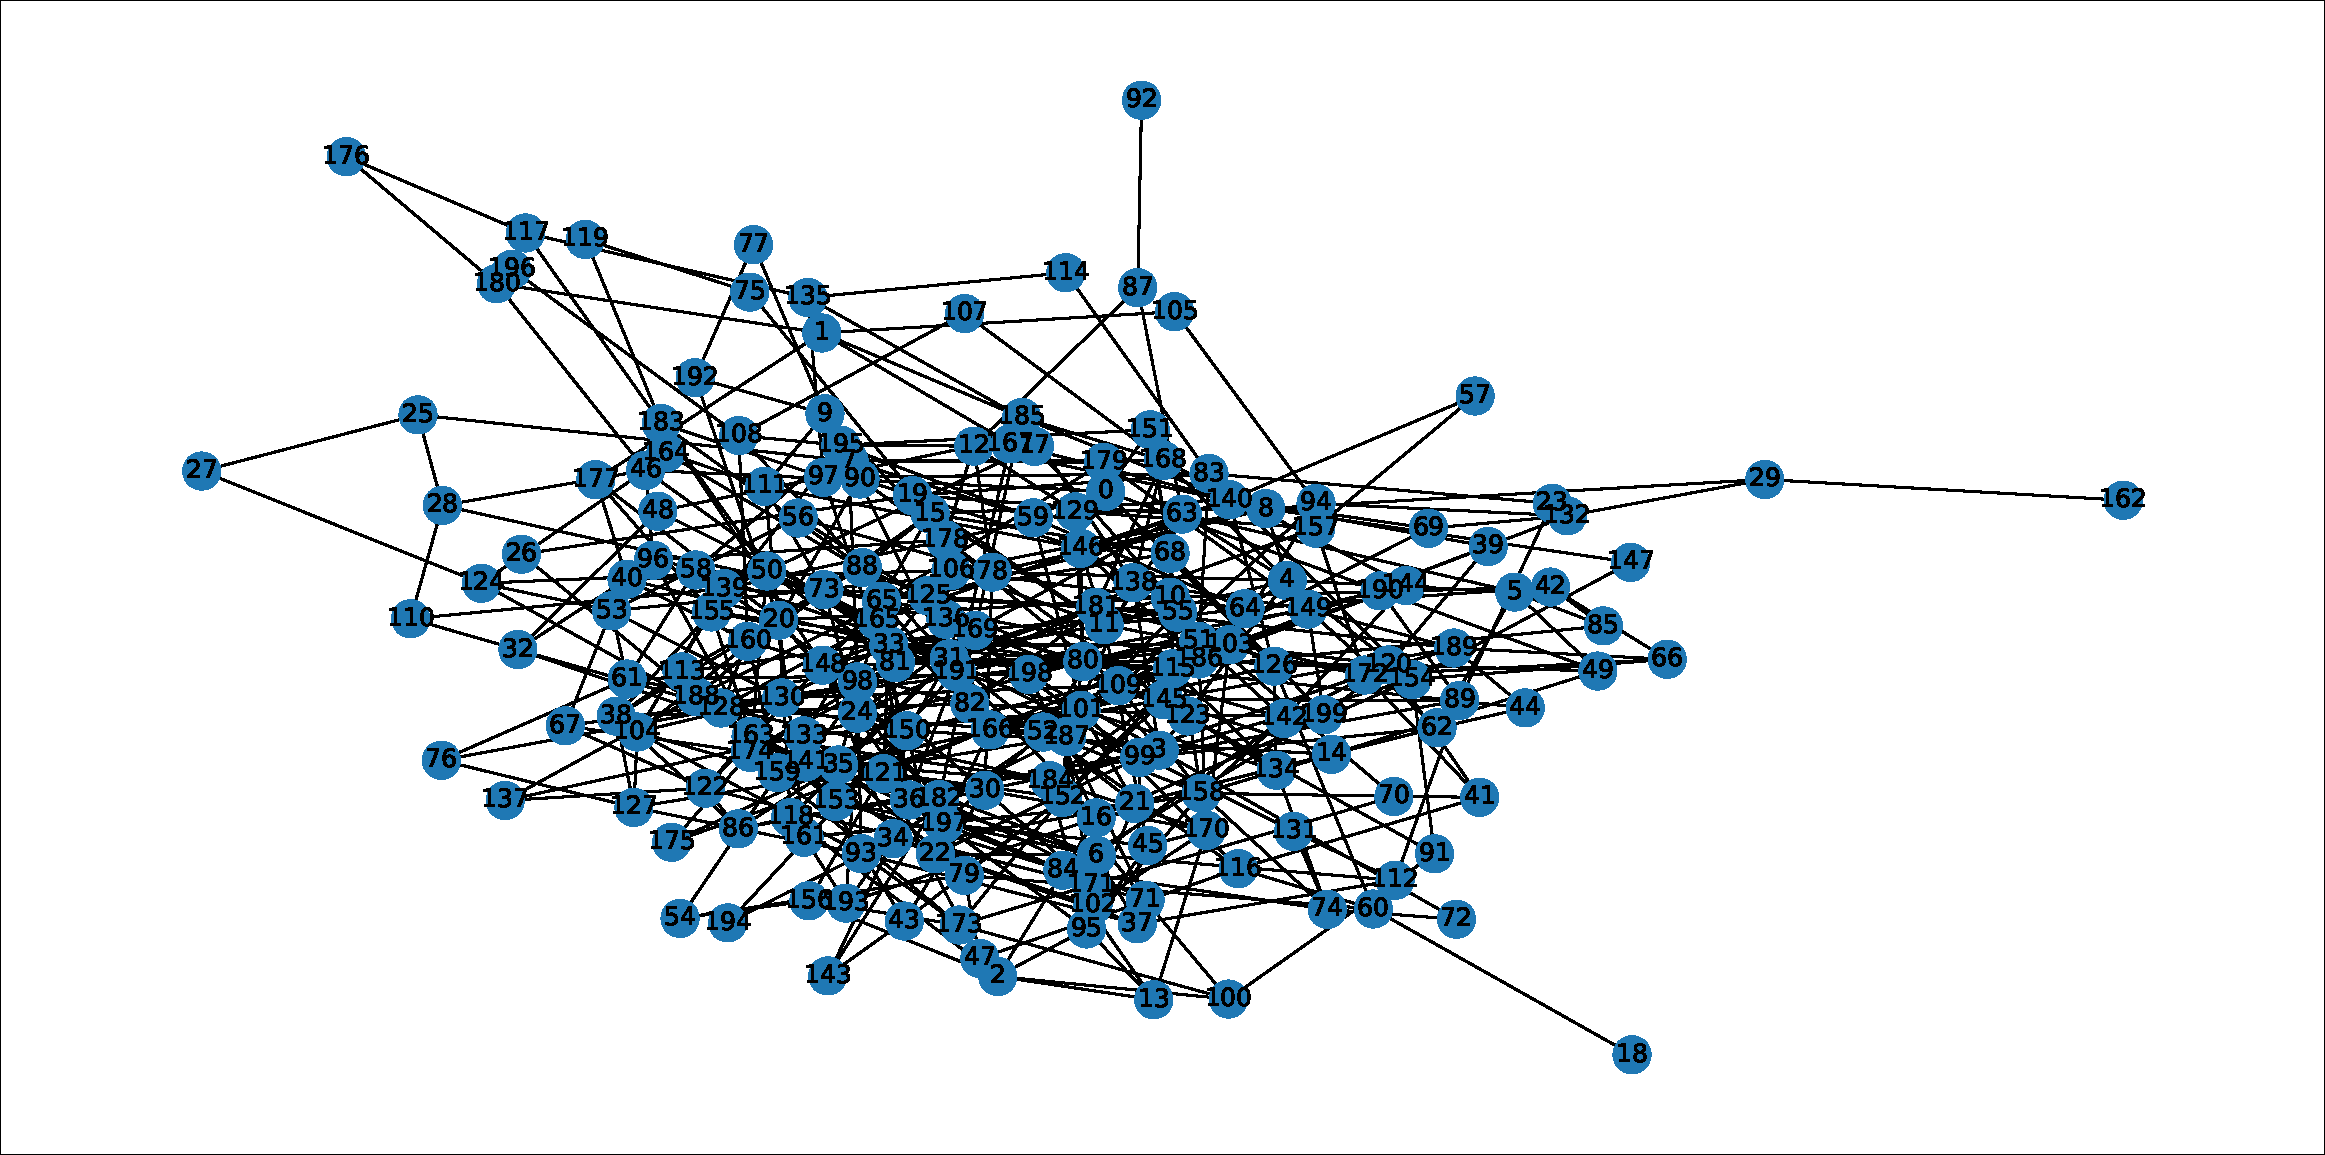
\includegraphics[width=\linewidth]{images/erdos_renyi/n200_p0.02649158683274018_0.pdf}
        \end{minipage}\hfill
        \begin{minipage}{0.32\textwidth}
            \centering
            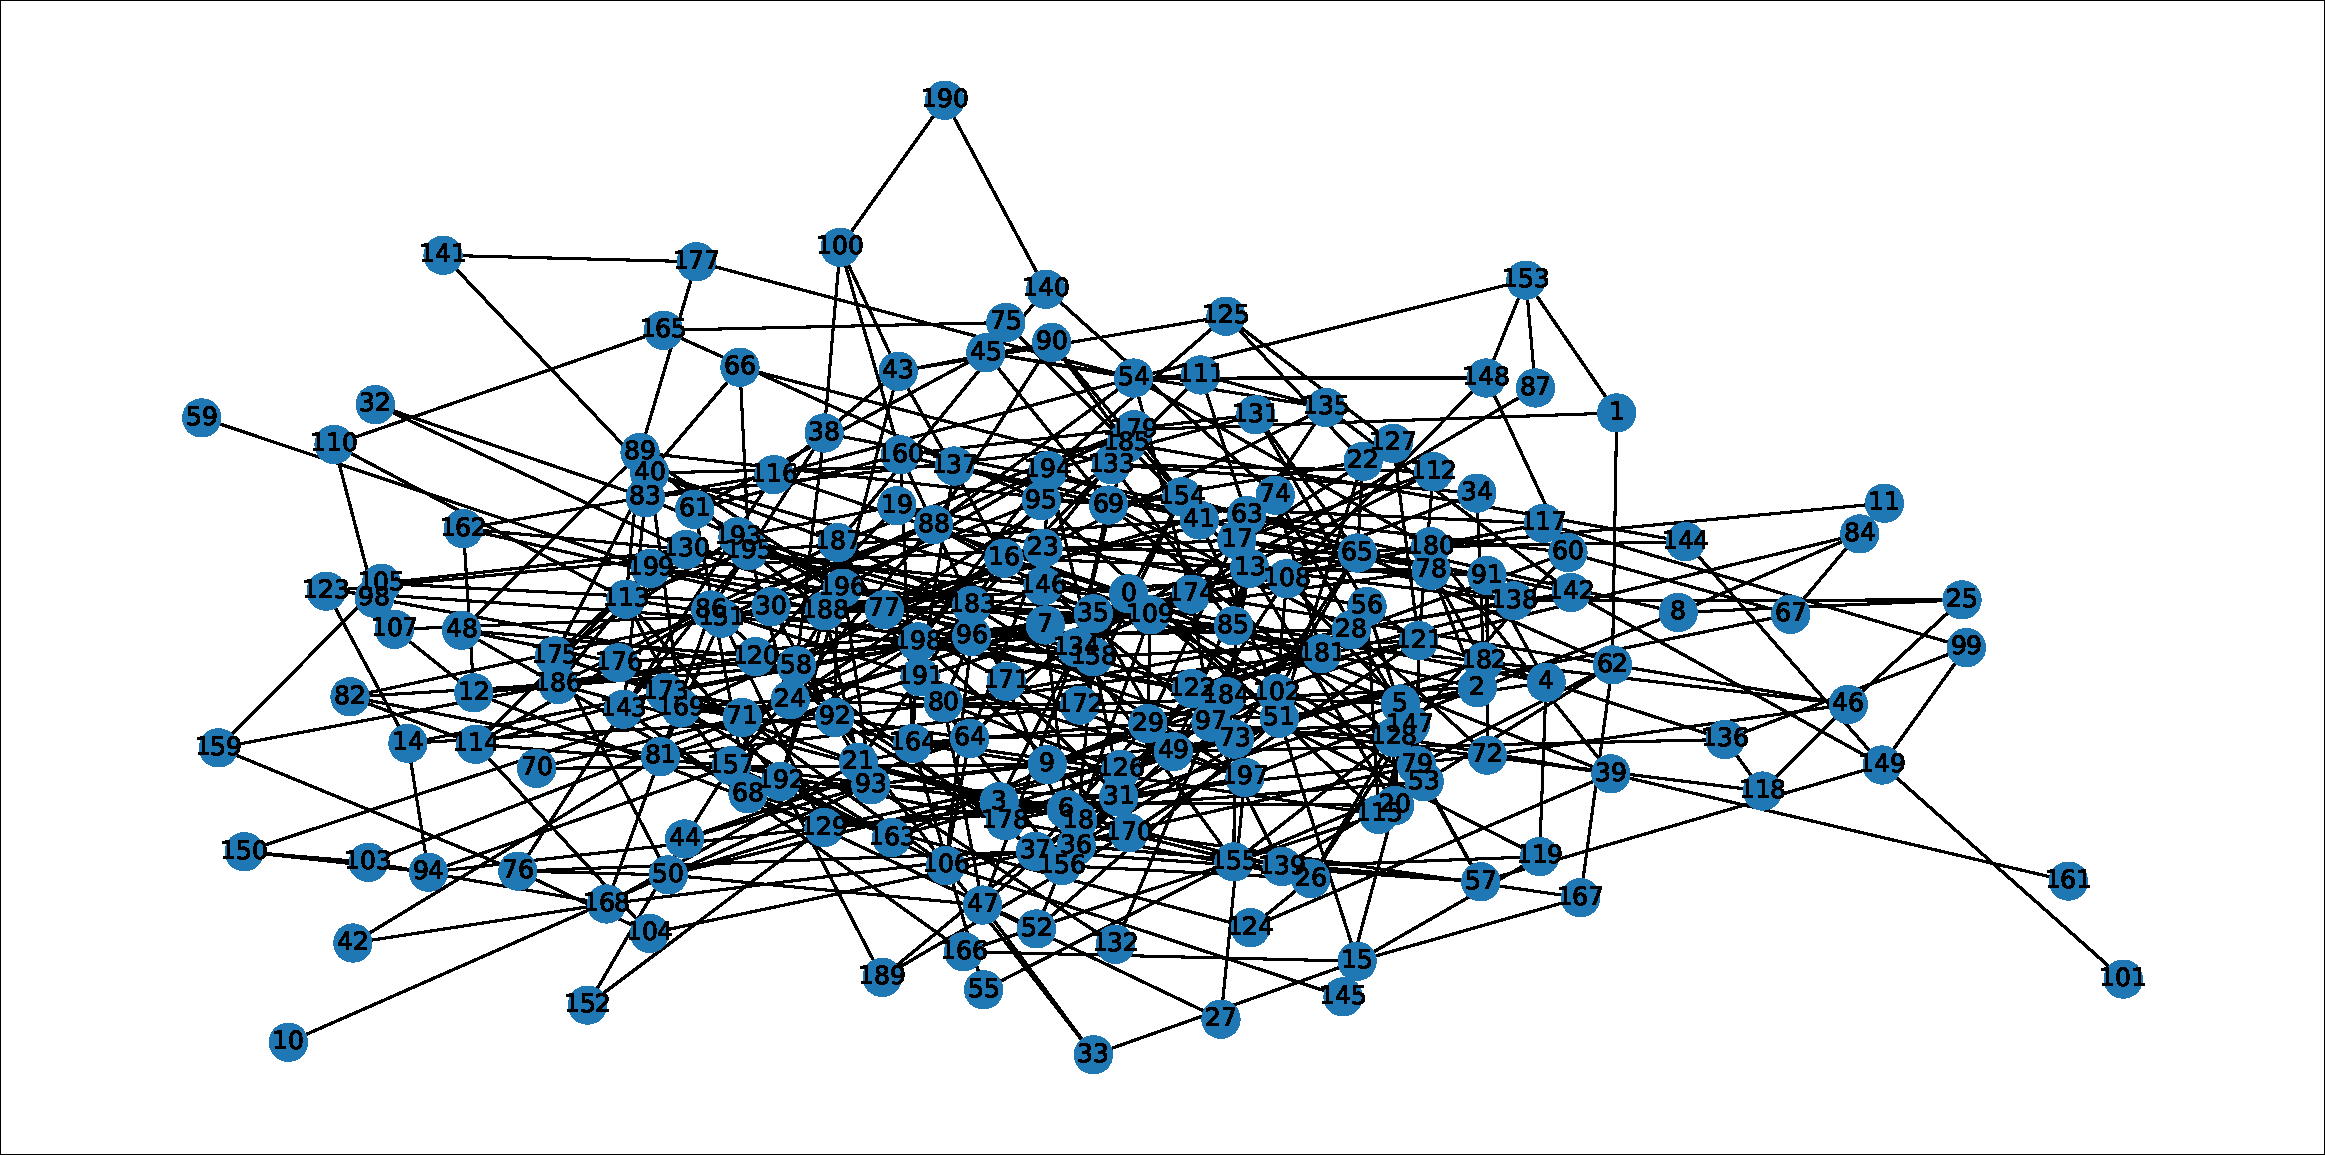
\includegraphics[width=\linewidth]{images/erdos_renyi/n200_p0.02649158683274018_1.pdf}
        \end{minipage}\hfill
        \begin{minipage}{0.32\textwidth}
            \centering
            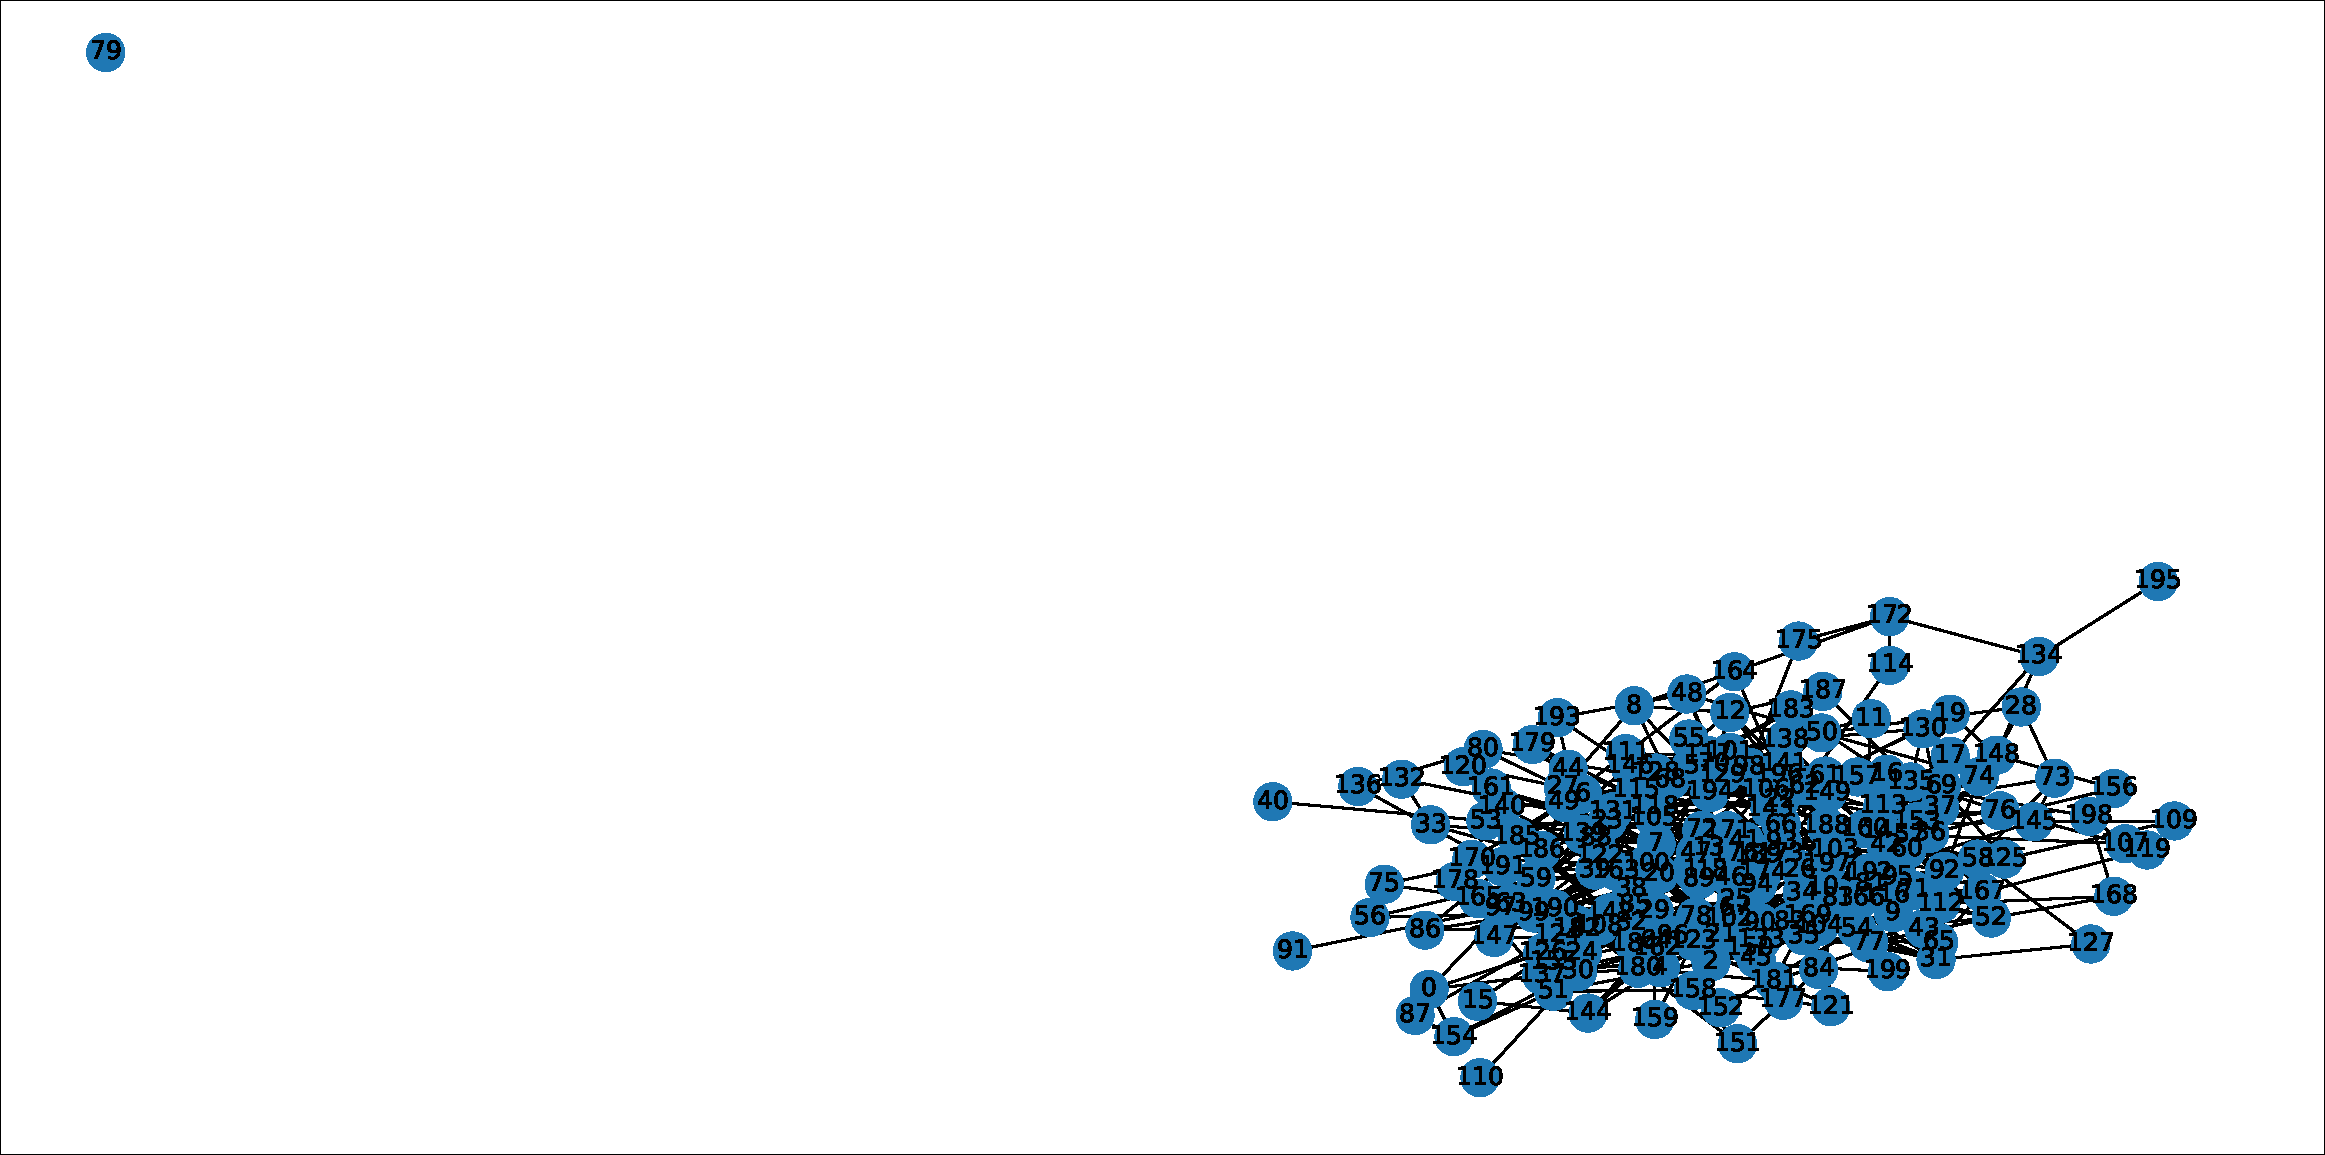
\includegraphics[width=\linewidth]{images/erdos_renyi/n200_p0.02649158683274018_2.pdf}
        \end{minipage}
        \caption{$n=200$, $p=0.02649$}
    \end{subfigure}

    \par\bigskip

    \begin{subfigure}{\textwidth}
        \centering
        \begin{minipage}{0.32\textwidth}
            \centering
            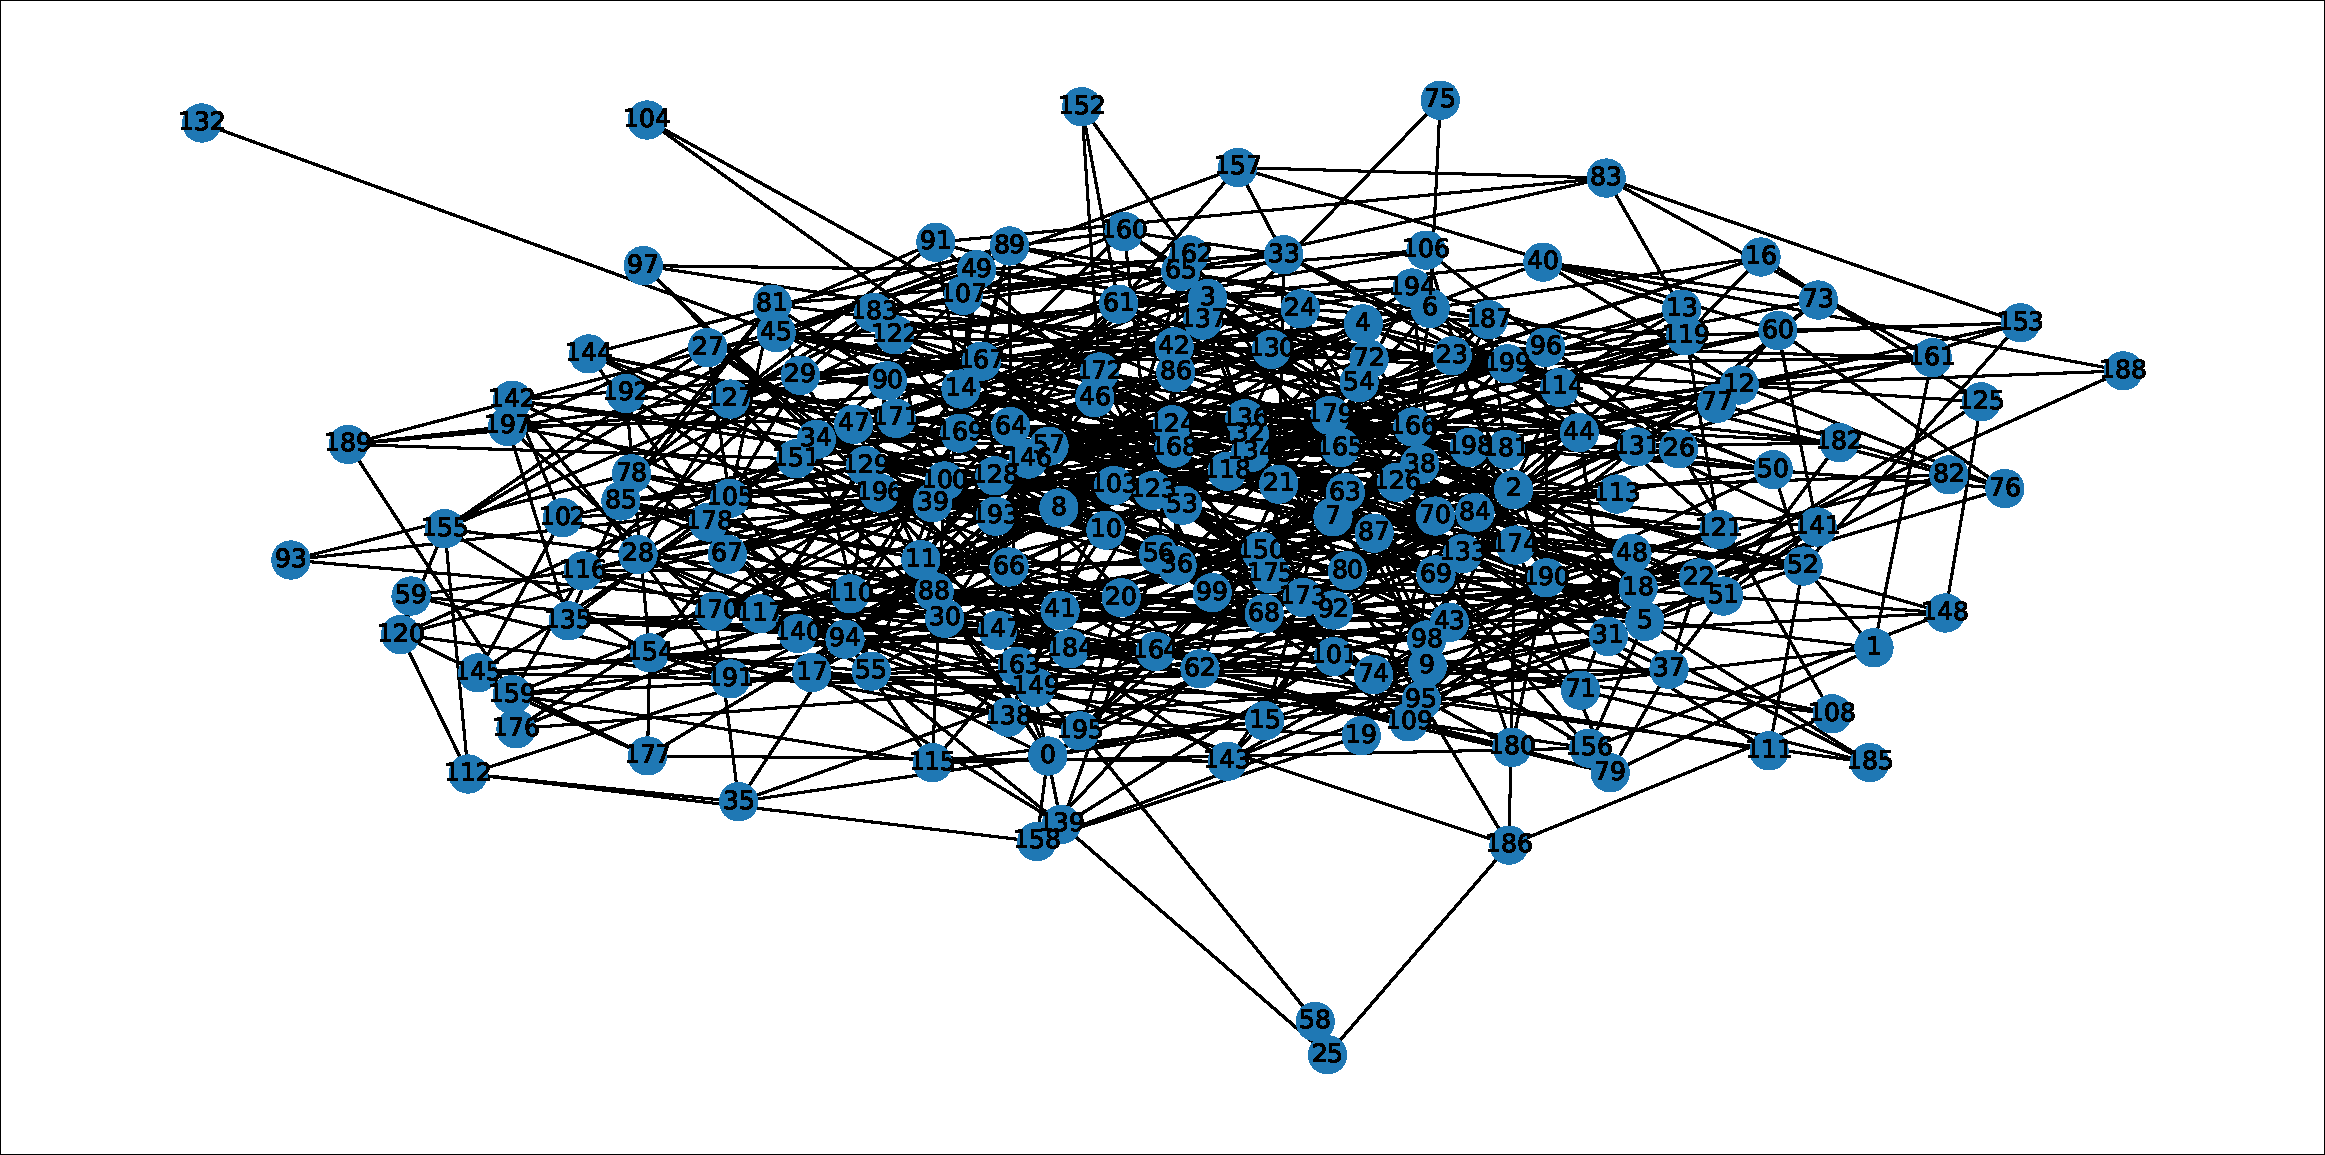
\includegraphics[width=\linewidth]{images/erdos_renyi/n200_p0.03649158683274018_0.pdf}
        \end{minipage}\hfill
        \begin{minipage}{0.32\textwidth}
            \centering
            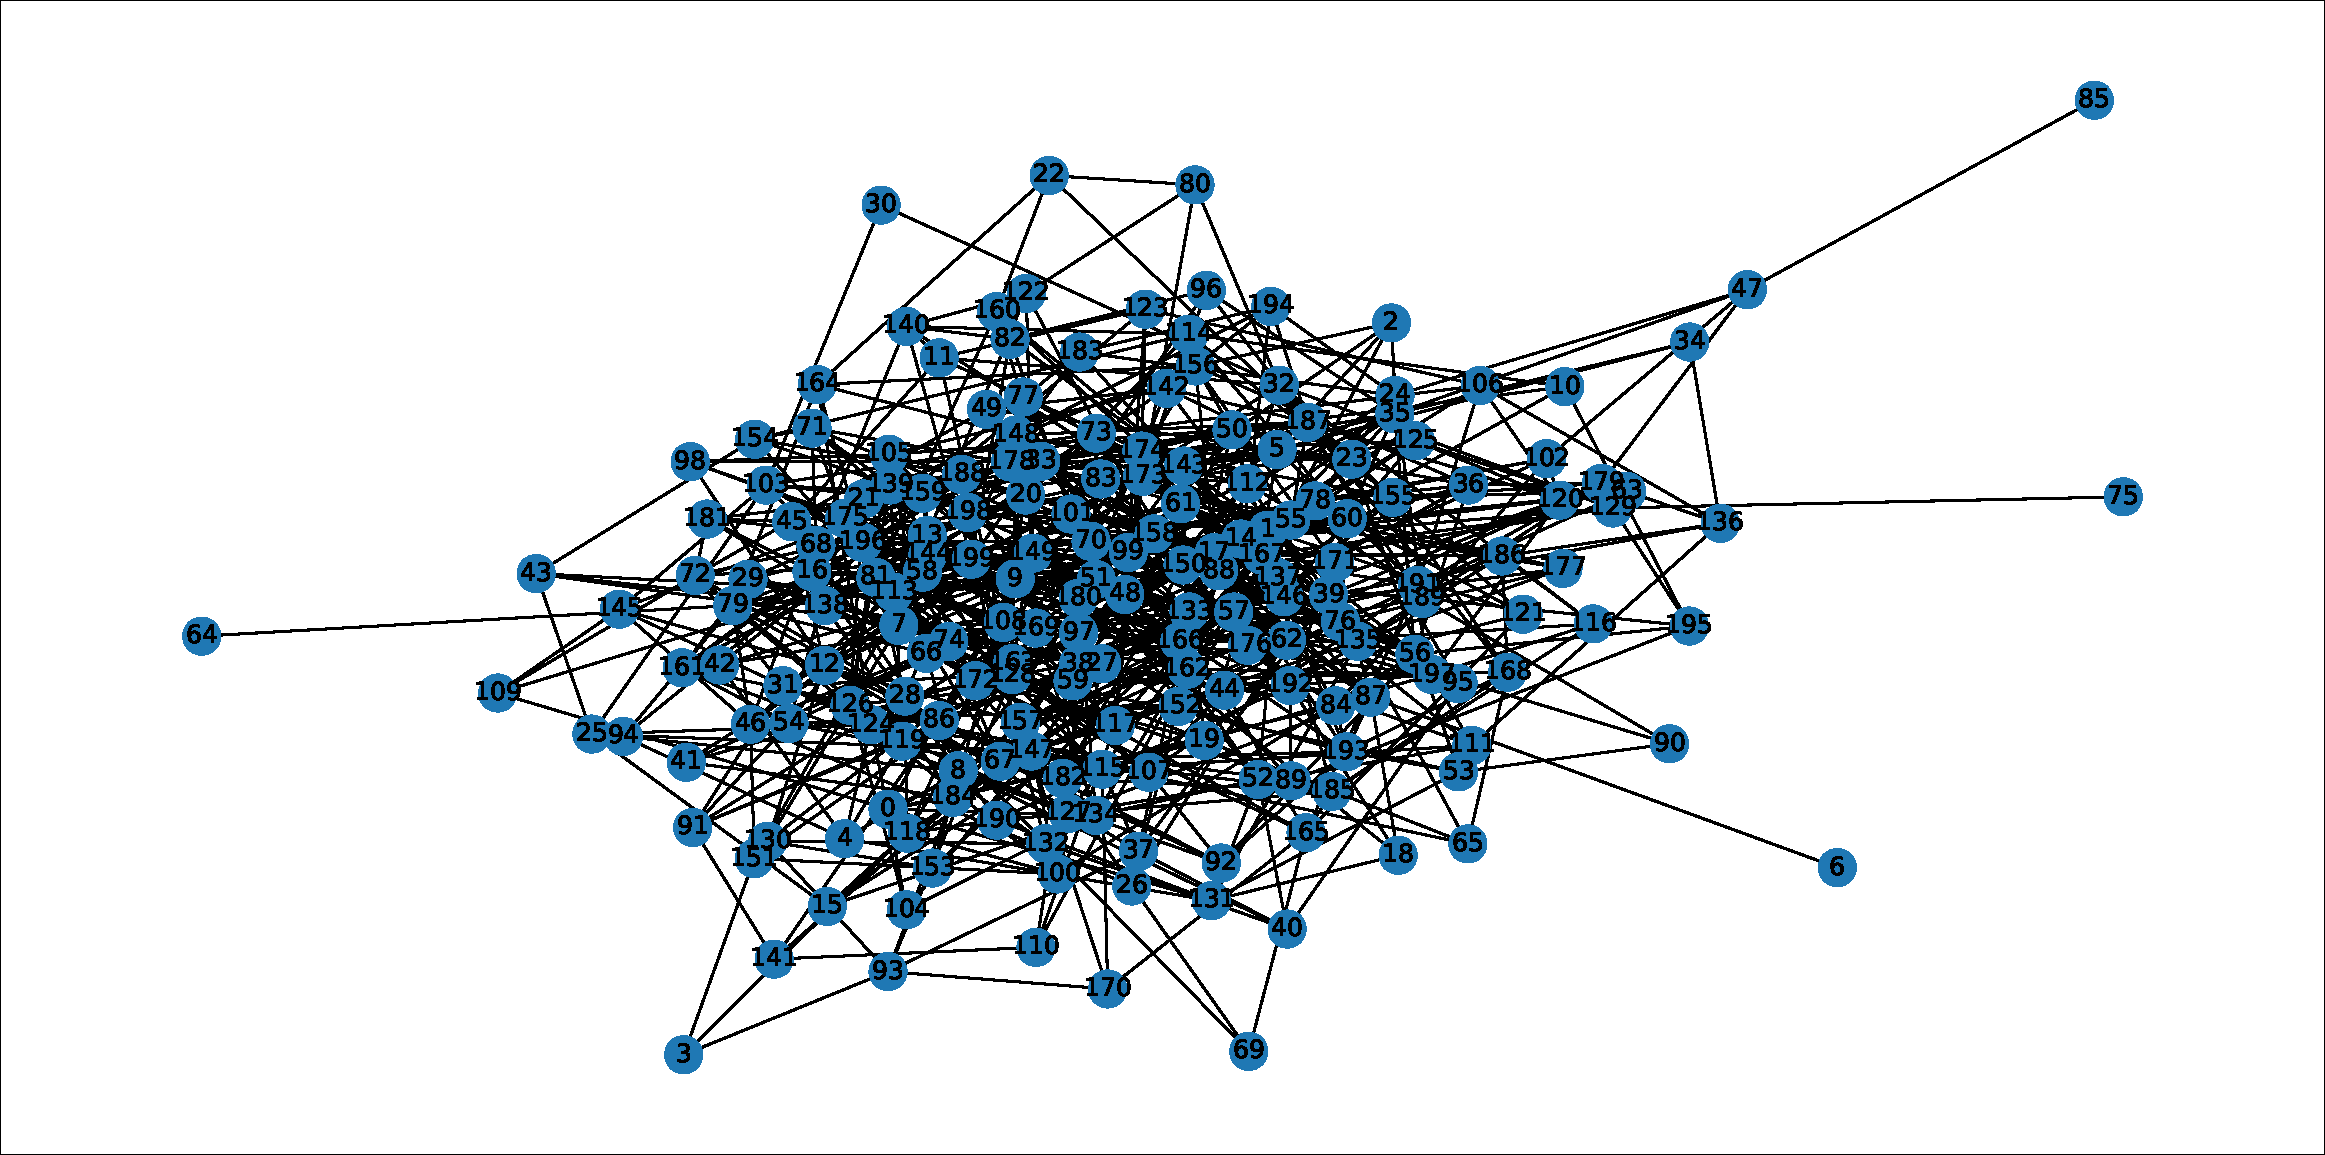
\includegraphics[width=\linewidth]{images/erdos_renyi/n200_p0.03649158683274018_1.pdf}
        \end{minipage}\hfill
        \begin{minipage}{0.32\textwidth}
            \centering
            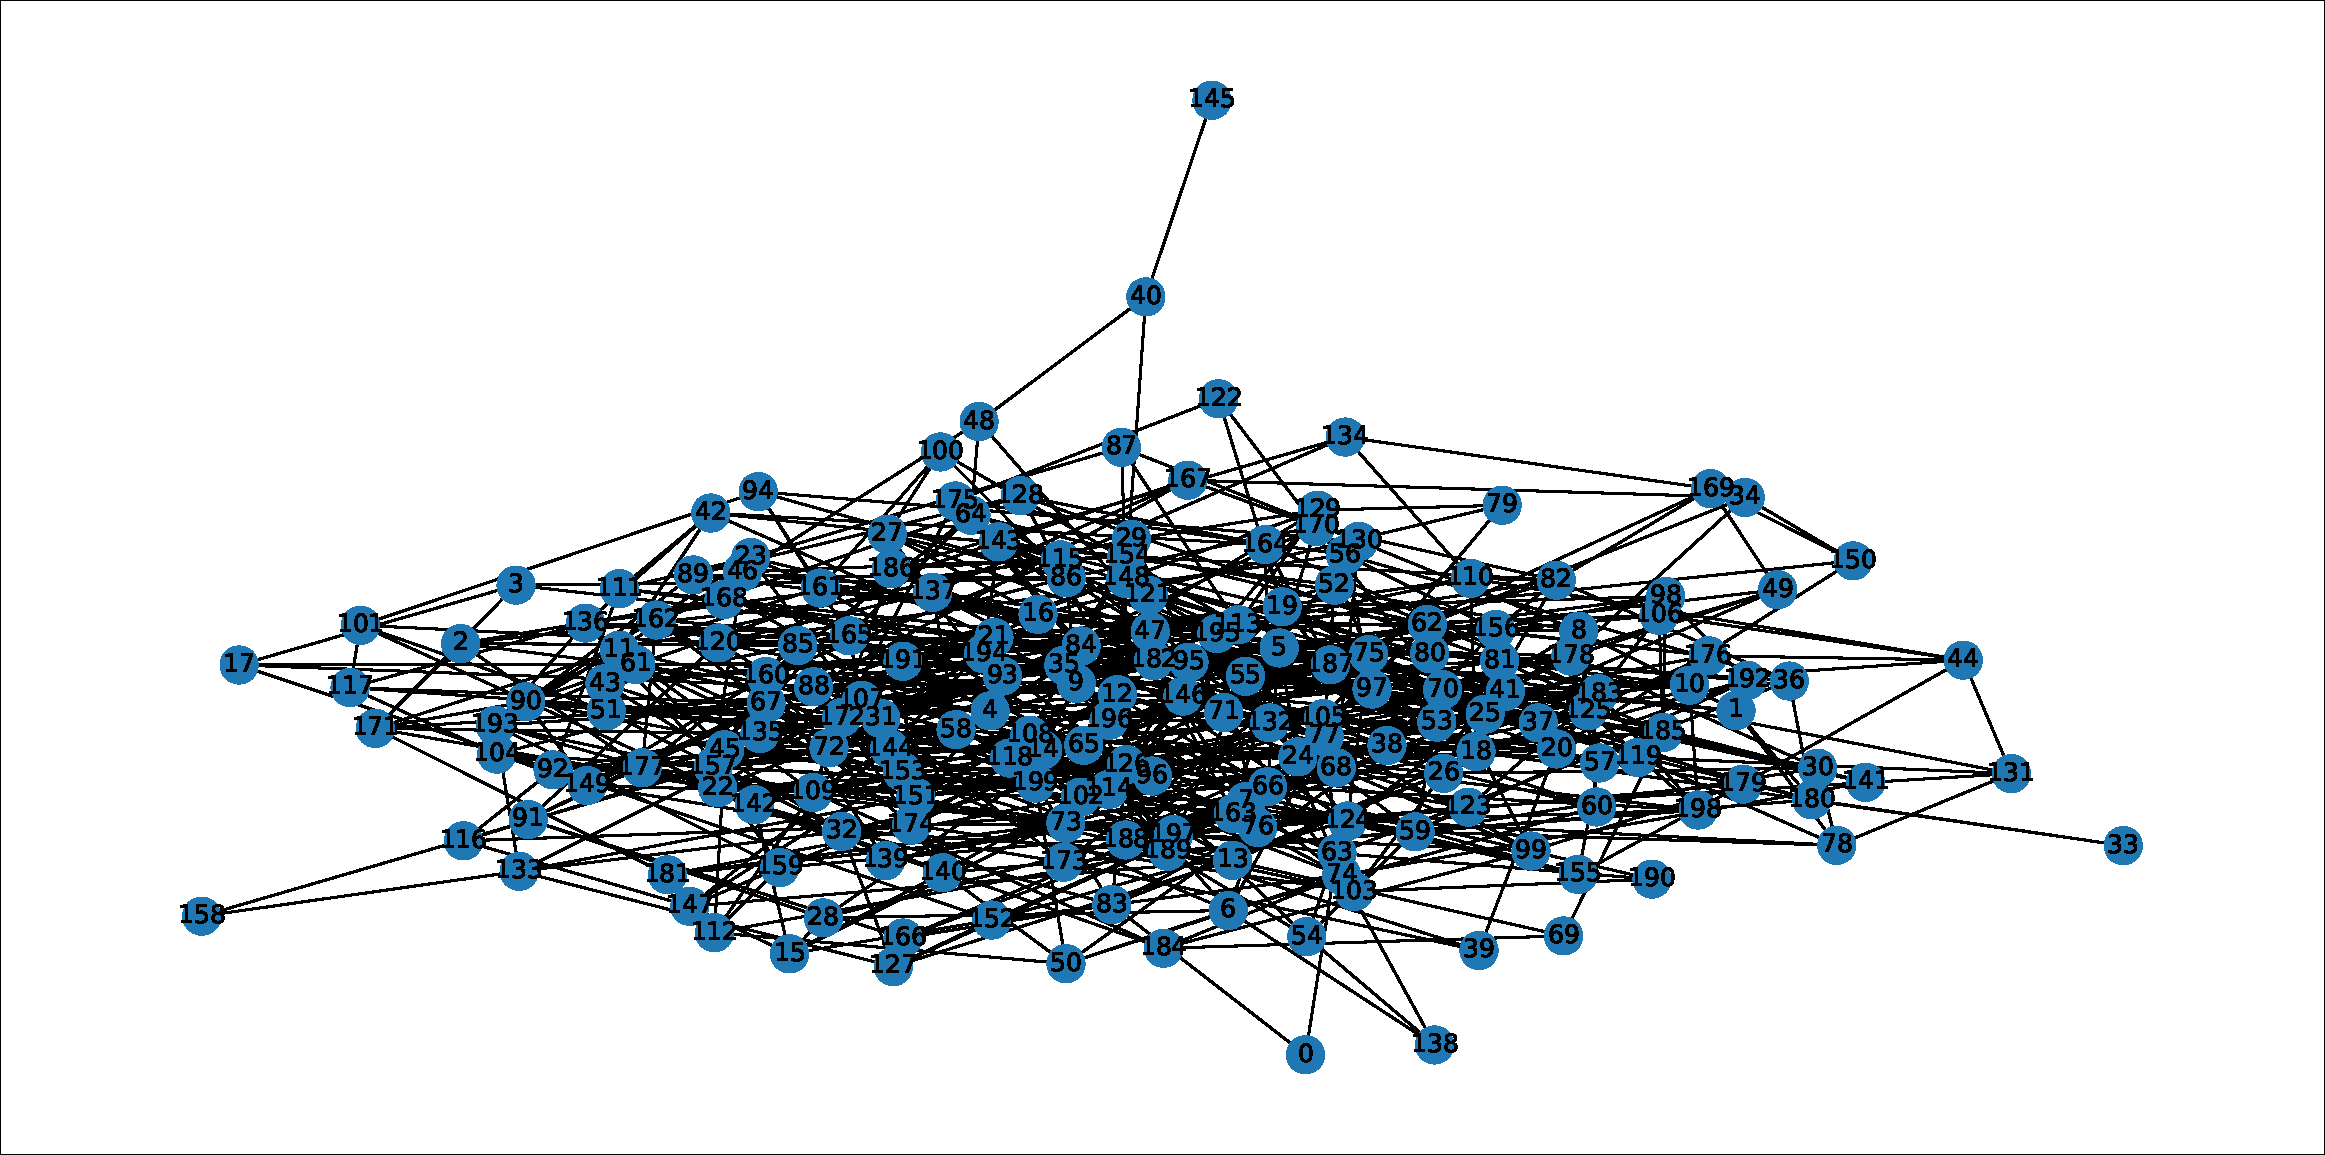
\includegraphics[width=\linewidth]{images/erdos_renyi/n200_p0.03649158683274018_2.pdf}
        \end{minipage}
        \caption{$n=200$, $p=0.03649$}
    \end{subfigure}

    \caption{Nueve realizaciones de grafos ER con $n=200$ y tres valores de $p$ alrededor del umbral de conectividad $p \approx \ln()/n$. }
    \label{fig:er_threshold}
\end{figure}

En la figura~\ref{fig:er_threshold} hacemos una validación empírica de esta propiedad, generando nueve grafos
con el algoritmo de ER con 200 nodos, variando la probabilidad $p$ alrededor del umbral de conectividad $p \approx \ln(n)/n \approx 0.02649$. Para cada valor de $p$ se generan tres grafos distintos.

La primera observación es que para valores de $p$ menores que el umbral de conectividad, el grafo es siempre disconexo, mientras que para valores de $p$ mayores que el umbral de conectividad, el grafo es siempre conexo. Cabe recalcar que las condiciones de las cotas~\eqref{eq:er_threshold_1} y~\eqref{eq:er_threshold_2} son probabilísticas, por lo que puede existir una realización del grafo que no cumpla con la condición, solo
que esto es altamente improbable. En el caso que $p$ es igual al umbral de conectividad, no podemos afirmar ningún comportamiento, y se ve reflejado en que algunos de los grafos son conexos y otros no. 

Otra característica a destacar, es que cuando el grafo ER no es conexo, las componentes que no pertenecen
a la componente conexa más grande, son nodos aislados. Esto esta relacionado a la tendencia de los grafos ER
a tener una componente gigante cuando $np>1$, condición que cumplen las 3 probabilidades elegidas.

\section{Grafos SBM}

Los grafos \emph{Stochastic Block Model} (SBM) son una extensión natural de los grafos ER, que busca solventar algunas de la limitaciones de los mismos. En particular,
los grafos ER no son capaces de generar comunidades, que es una característica importante en muchos grafos reales. Los grafos SBM solucionan este problema trabajando
con una matriz de probabilidad $Q$ simétrica, donde $Q_{ij}$ es la probabilidad de que un nodo del grupo $i$ se conecte con un nodo del grupo $j$. La cantidad de nodos 
en cada grupos son parámetros del modelo $n_i$.

\begin{figure}[htb]
    \centering
    \begin{subfigure}{0.49\textwidth}
        \centering
        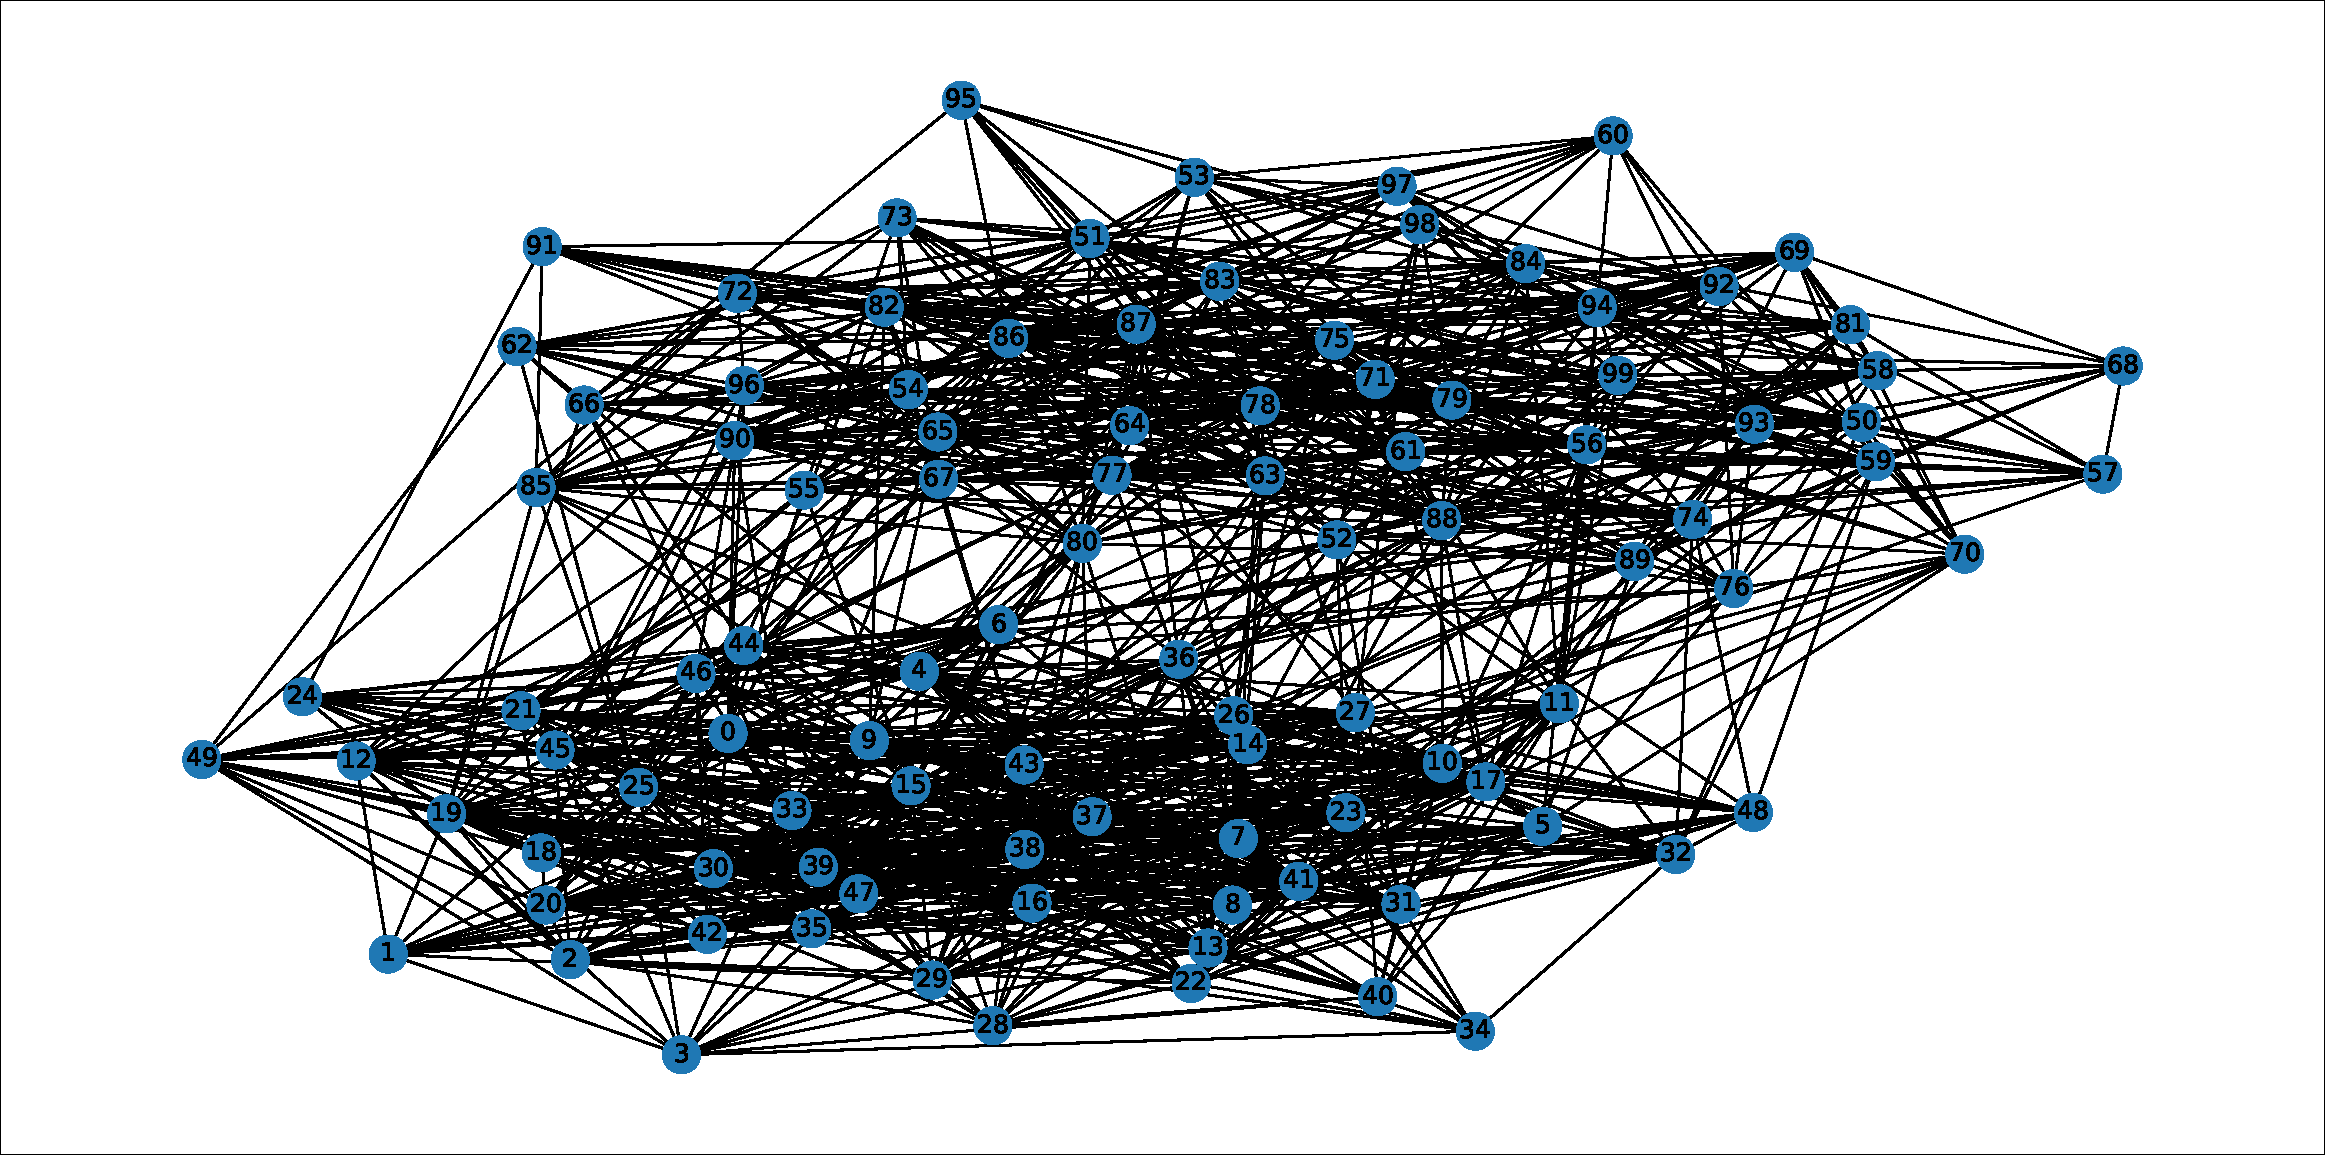
\includegraphics[width=\linewidth]{images/sbm/n50_0_0.421_0.279.pdf}
        \caption{SBM con valores propios $0.421$ y $0.279$, asociado a la matriz $Q_1$ \eqref{eq:sbm_matrices}.}
        \label{fig:sbm_eigenvalues_reference}
    \end{subfigure}
    \hfill
    \begin{subfigure}{0.49\textwidth}
        \centering
        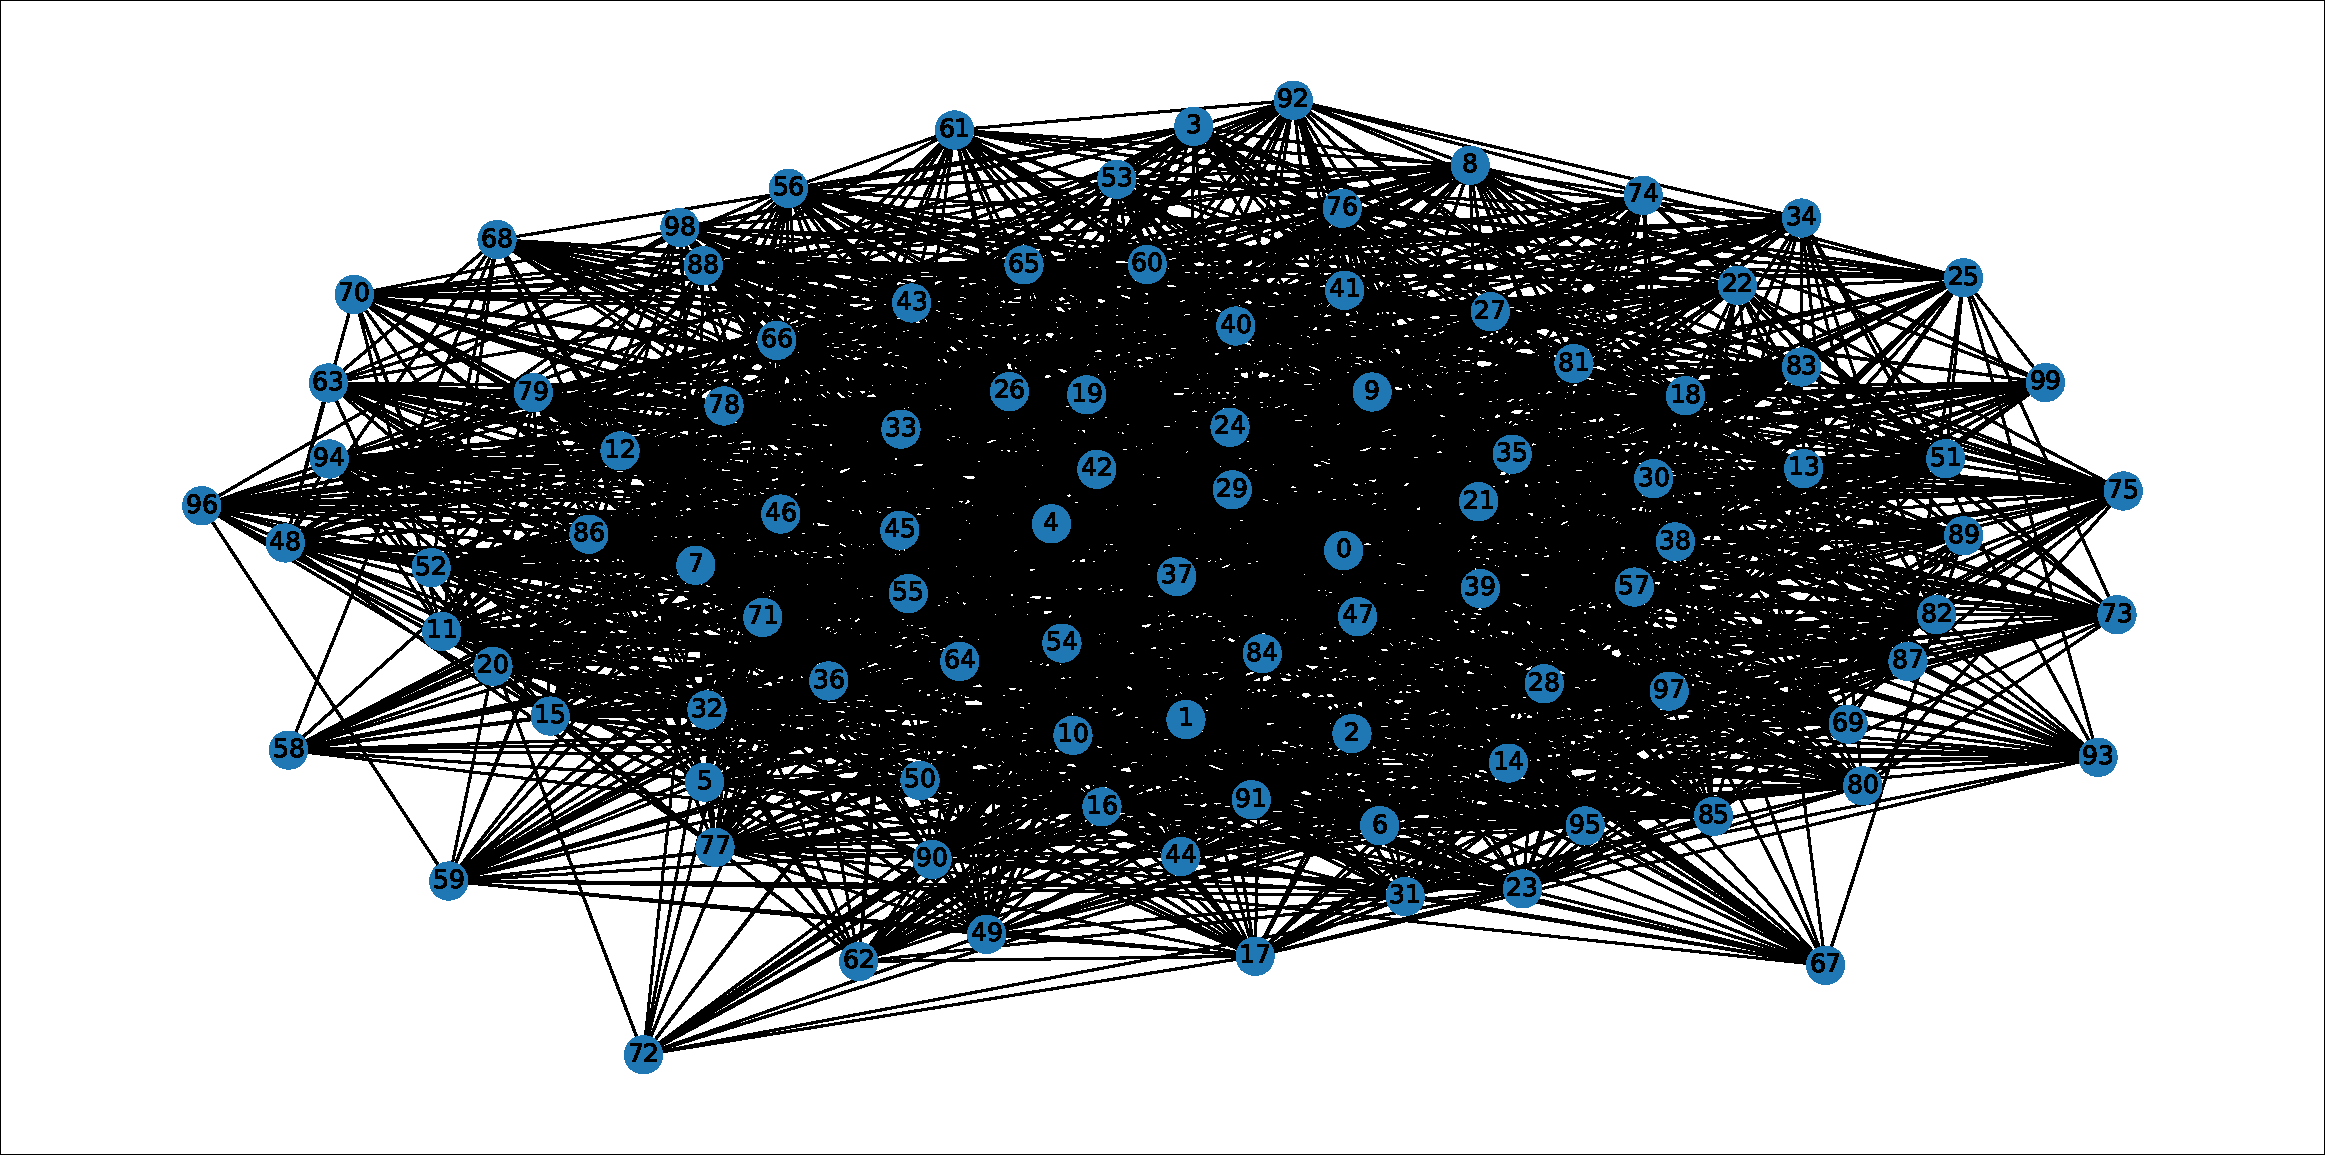
\includegraphics[width=\linewidth]{images/sbm/n50_1_0.652_-0.352.pdf}
        \caption{SBM con valores propios $0.652$ y $-0.352$, asociado a la matriz $Q_2$ \eqref{eq:sbm_matrices}.}
        \label{fig:sbm_eigenvalues_negative}
    \end{subfigure}
    \par\bigskip
    \begin{subfigure}{0.49\textwidth}
        \centering
        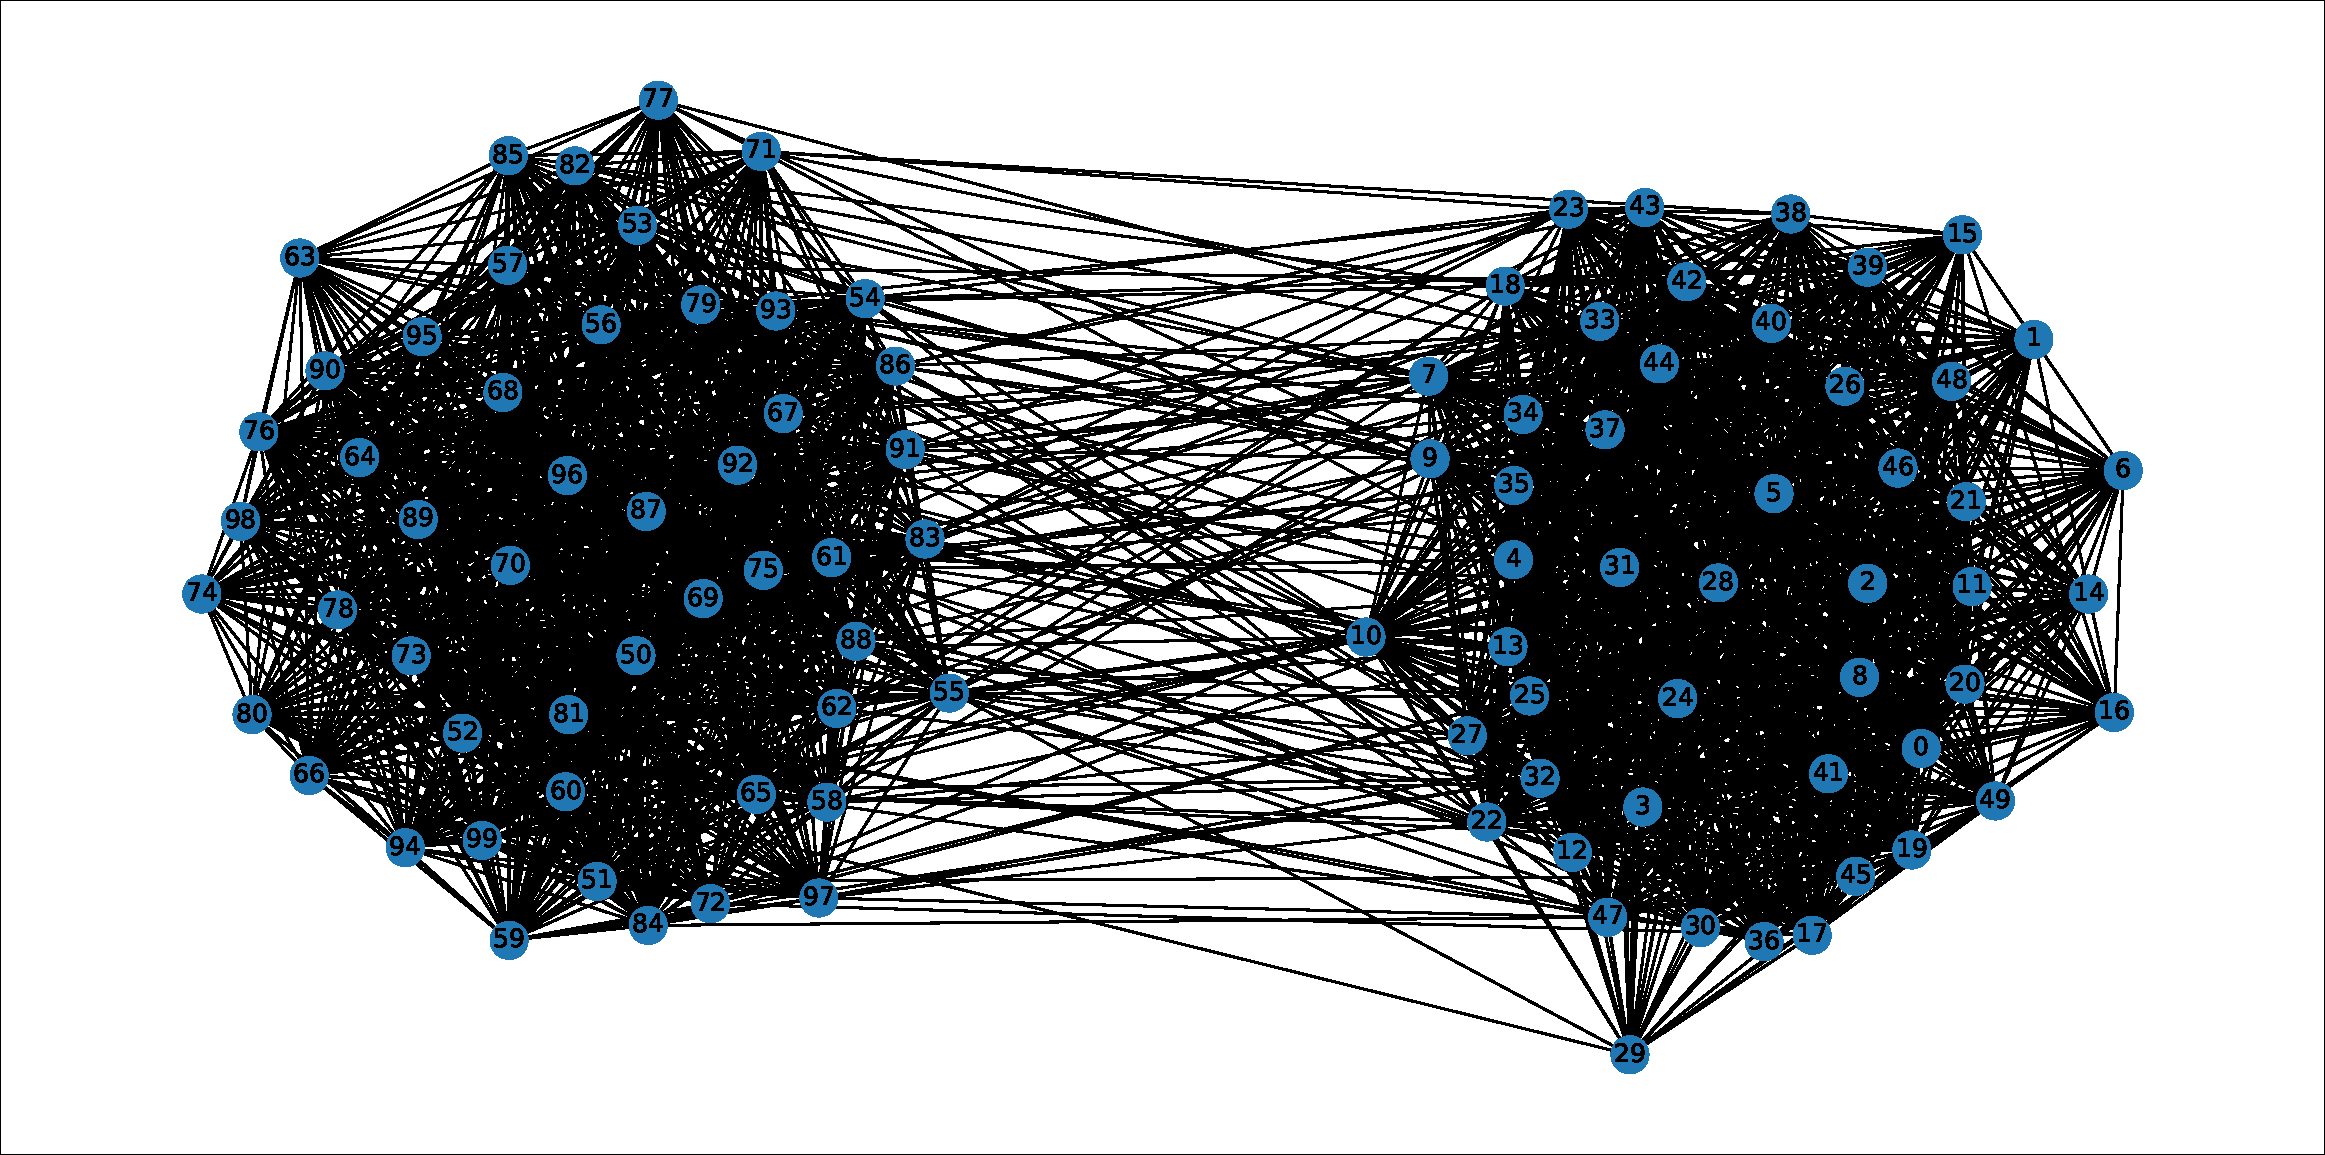
\includegraphics[width=\linewidth]{images/sbm/n50_2_0.85_0.75.pdf}
        \caption{SBM con valores propios $0.85$ y $0.75$, asociado a la matriz $Q_3$ \eqref{eq:sbm_matrices}.}
        \label{fig:sbm_eigenvalues_big}
    \end{subfigure}
    \caption{Tres realizaciones de un grafo SBM con dos comunidades de igual tamaño, y dos valores distintos de $Q$.}
    \label{fig:sbm_eigenvalues}
\end{figure}

Analizemos el impacto de los vectores propios de la matriz $Q$ en el grafo generado. Por simplicidad, trabajaremos con dos comunidades de igual tamaño $n_1=n_2=50$.
En la figura~\ref{fig:sbm_eigenvalues} se muestran tres realizaciones de un grafo SBM, con las matrices:
\begin{equation}
    \label{eq:sbm_matrices}
    Q_1 = \left( \begin{matrix}
        0.4 & 0.05 \\
        0.05 & 0.3
    \end{matrix} \right) \quad
    Q_2 = \left( \begin{matrix}
        0.2 & 0.5 \\
        0.5 & 0.1
    \end{matrix} \right) \quad
    Q_3 = \left( \begin{matrix}
        0.8 & 0.05 \\
        0.05 & 0.8
    \end{matrix} \right)
\end{equation}

Intuitivamente, los valores de la diagonal indican que tan densamente conectada esta una comunidad, mientras que los valores fuera indican que tanto se conectan 
entre comunidades. Viendo la figura~\ref{fig:sbm_eigenvalues_negative} vemos el resultado de la matriz $Q_2$, donde el valor de intraconexión de una comunidad es 
similar al valor de interconexión entre comunidades. Esto deriva en un valor propio negativo, y en un grafo con una sola comunidad.

En los otros dos casos, tenemos matrices $Q$ con valores propios positivos. Podemos notar como las comunidades de la figura~\ref{fig:sbm_eigenvalues_big} son muchas 
densas que en la figura~\ref{fig:sbm_eigenvalues_reference}, lo cual es esperable dada la matriz $Q$ asociada. Si observamos los valores propios, vemos que son 
mayores para $Q_3$, de lo que podemos concluir que hay una correlación entre la densidad de la comunidad y el valor propio asociado.

En resumen, los valores propios de la matriz $Q$ son indicadores de la cantidad y densidad de las comunidades del grafo generado, donde la cantidad de valores
propios positivos es igual a la cantidad de comunidades. Apliquemos este resultado a una matriz $Q$ con $n=[45, 5, 45, 5]$:
\begin{equation}
    \label{eq:sbm_4x4_matrix}
    Q = \begin{pmatrix}
        0.05 & 0.9 & 0.0 & 0.0 \\
        0.9 & 0.8 & 0.0 & 0.5 \\
        0.0 & 0.0 & 0.05 & 0.9 \\
        0.0 & 0.5 & 0.9 & 0.9
    \end{pmatrix}
\end{equation}
Antes que nada, intuitivamente podemos ver que hay comunidades que no van a existir, puesto que su valor en la diagonal es menor que los valores
fuera de la diagonal. Calculando los valores propios de la matriz $Q$, obtenemos:
\begin{equation}
    \label{eq:sbm_4x4_eigenvalues}
    \lambda_1 = 1.81, \quad\lambda_2 = 1.11, \quad\lambda_3 = -0.71, \quad\lambda_4 = -0.41
\end{equation}
Podemos ver que hay dos valores propios positivos, y dos negativos. Por lo tanto, deberíamos obtener un grafo con dos comunidades. 
La figura~\ref{fig:sbm_4x4_eigenvalues} muestra el resultado de la generación, donde efectivamente observamos que el grafo resultante
tiene dos comunidades. En la figura~\ref{fig:sbm_4x4_adj_matrix} podemos ver la matriz de adyacencia del grafo resultante, donde se entiende
la intuición que planteamos incialmente: la conexión intracomunidad (valor de la diagonal) tiene que ser suficientemente mayor que la conexión intercomunidad (valor fuera de la diagonal) para que se forme una comunidad.

\begin{figure}[htb]
    \centering
    \begin{subfigure}{0.8\textwidth}
        \centering
        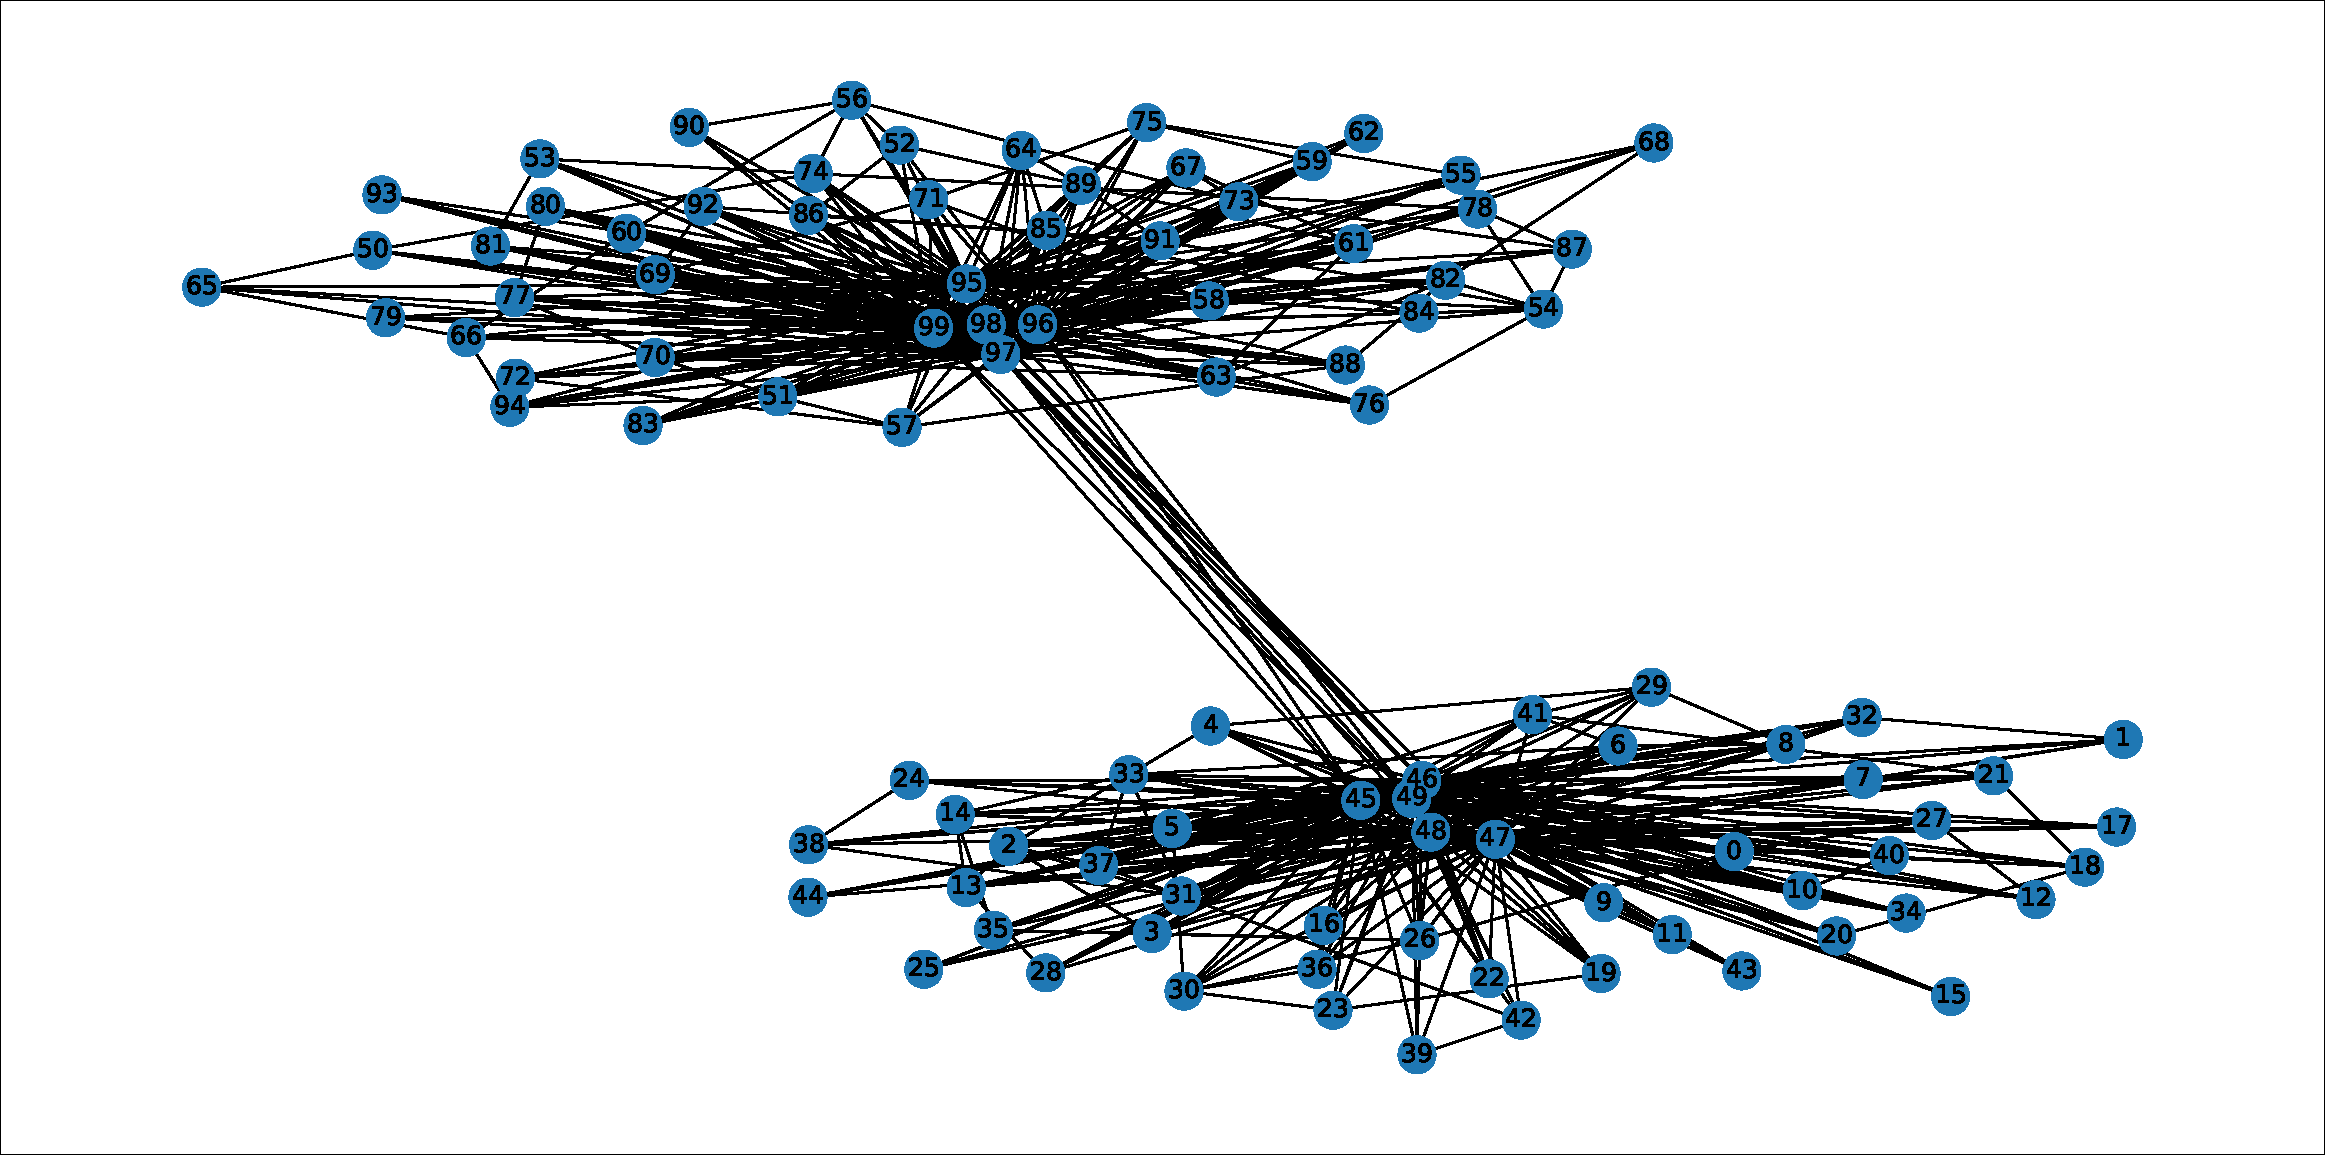
\includegraphics[width=\linewidth]{images/sbm/sbm_4n.pdf}
        \caption{Realización del grafo SBM.}
        \label{fig:sbm_4x4_eigenvalues}
    \end{subfigure}
    \par\bigskip
    \begin{subfigure}{0.6\textwidth}
        \centering
        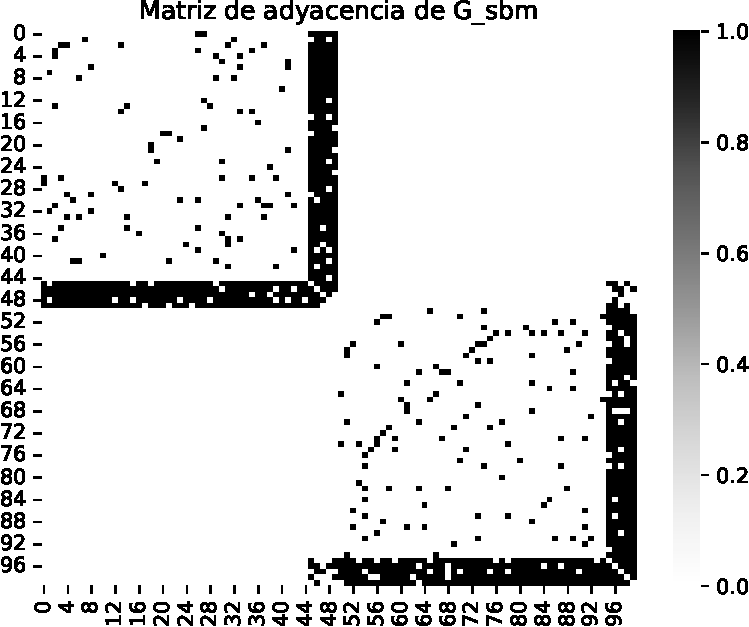
\includegraphics[width=\linewidth]{images/sbm/sbm_4n_adj_matrix.pdf}
        \caption{Matriz de adyacencia del grafo SBM.}
        \label{fig:sbm_4x4_adj_matrix}
    \end{subfigure}
    \caption{SBM con valores propios \eqref{eq:sbm_4x4_eigenvalues}, asociado a la matriz $Q$ \eqref{eq:sbm_4x4_matrix}.}
    \label{fig:sbm_4x4_generation}
\end{figure}

\section{Grafos RDPG}

\subsection{definicion}

\subsection{inferencia}

\subsection{Clustering }

\section{Ejemplo real}

\FloatBarrier
\bibliography{refs.bib}
\bibliographystyle{plain}

\end{document}